% Author: Joshua Sello

\documentclass{elsarticle}
\usepackage[margin=2.5cm]{geometry}
\usepackage{amsmath}
\usepackage{booktabs}
\usepackage{tabularx}
\usepackage{array}
\usepackage{xcolor}

% Model notation
\newcommand{\MR}{\ensuremath{M_\mathrm{R}}}
\newcommand{\MA}{\ensuremath{M_\mathrm{A}}}

% TODO: Change this when journal is selected.
\journal{Journal with Giga Impact Factor}

\begin{document}

\begin{frontmatter}

\title{Does Behavioural Fidelity Change Charging Infrastructure Decisions? Data Replay and Agent-Based Simulation for Minibus-Taxi Electrification in Cape Town}

\author[aff1]{J.~T. Sello\corref{cor1}}
\ead{jtsello@sun.ac.za}
\author[aff1,aff2,aff3]{M.~J. Booysen}
\ead{mjbooysen@sun.ac.za}

\cortext[cor1]{Corresponding author}

\affiliation[aff1]{organization={Electrical and Electronic Engineering, Stellenbosch University},
                   country={South Africa}}
\affiliation[aff2]{organization={Industrial Engineering, Stellenbosch University},
                   country={South Africa}}
\affiliation[aff3]{organization={Department of Computing and Technology, Uganda Christian University},
                   country={Uganda}}

\begin{abstract}
    % Discuss > Problem -> Electrification couples paratransit mobility, batteries, chargers and the grid, and drivers control the mobility. Planning studies either replay observed mobility or simulate driver decisions.
    % Discuss > Design -> Three minibus-taxi communities in Cape Town, selected by a frozen rule from 11 communities that are found in router GPS data.
    % Discuss > Methods -> Data replay (\MR) and a mixed-fleet agent-based model (\MA) with the full corridor population; every charging design is evaluated in both models.
    % Discuss > Results -> One sentence per RQ: outcome difference (E1), design difference (E2--E4), cost of the replay design and EV passenger loss (E5), consistency over communities (E6, synthesis).
    % Discuss > Implication -> When driver agency matters for pilot charging infrastructure.
    \textcolor{red}{Complete abstract.}
\end{abstract}

\begin{keyword}
    paratransit \sep minibus taxi \sep electrification \sep agent-based modelling \sep data replay \sep charging infrastructure \sep vehicle communities \sep mixed fleet \sep multi-objective design evaluation \sep Cape Town
\end{keyword}

\end{frontmatter}

% --------------------------------------------------
%   Introduction
% --------------------------------------------------

\section{Introduction}
\textcolor{red}{TODO: Complete introduction.}

\subsection{Paratransit electrification as a coupled planning problem}

% Discuss > Establish that electrification couples previously weakly coupled systems: mobility <-> battery <-> charging <-> grid. and that paratransit adds another important coupling: electrification constraints <-> driver behaviour.
% - Slow charging, limited range and finite chargers create opportunity costs that did not exist in the same form for ICE vehicles.

Paratransit systems, such as minibus taxis, are a critical component of urban mobility in many cities, particularly in developing countries. As global efforts to reduce greenhouse gas emissions intensify, the electrification of these systems has become a focal point for sustainable urban transport planning~\cite{nasac2024_decarbonising_transport_in_africa, bankole2026_electrifying_paratransit_ssa}. However, the transition from internal combustion engine (ICE) vehicles to electric vehicles (EVs) introduces a complex set of interdependencies that were previously weakly coupled. Specifically, the mobility of vehicles is now closely linked to vehicle drive-train efficiency, battery capacity, and charging infrastructure, which in turn affects the electrical grid and drivers' ability to service passenger demand~\cite{booysen2025_sys_of_sys_em_planning}. This coupling creates new challenges for planning and operation, as the limitations of electric vehicles (EVs), such as slower charging times and limited range, changes the operational status quo, introducing opportunity costs that were not present for internal combustion engine (ICE) vehicles~\cite{}. When investigating the electrification of paratransit system, it is therefore essential that the planning models account for the interactions between these systems, as well as the adaptive behaviour of drivers who respond to these constraints in their operational decisions~\cite{}.

% Discuss > Driver agency -> Drivers control much of the underlying mobility through decisions about where, when and how long to operate.

In South Africa, minibus-taxi drivers have significant agency over their operational decisions, including where, when, and how long to operate~\cite{}. This agency allows drivers to adapt their behaviour in response to the constraints imposed by electrification, such as limited range and charging availability. As a result, the success of electrification initiatives is not solely dependent on the technical feasibility of EVs but also on how drivers respond to these new operational constraints. Understanding and modelling driver behaviour is therefore crucial for accurately predicting the outcomes of electrification and for designing effective charging infrastructure that meets both operational and passenger demand requirements.

% Discuss > Conclude -> Therefore infrastructure requirements may depend on whether mobility is treated as: fixed; or adaptive.
Therefore, the planning of charging infrastructure for paratransit electrification must consider whether mobility should be treated as fixed or adaptive. Fixed-mobility models, otherwise termed ``data-replay models'', assume that observed vehicle activity will largely persist after electrification, while adaptive-mobility models account for the potential changes in driver behaviour in response to introduced constraints. The choice between these two paradigms can significantly influence the predicted outcomes of electrification and the resulting infrastructure requirements, highlighting the importance of incorporating behavioural fidelity into planning models.


\subsection{Modelling paratransit: the tale of two paradigms}
% Discuss > Rehash the discussion had in the Gaurav paper + Booysen et al. sys-of-sys paper. Establish that the modelling of paratransit is a complex problem, and that the modelling of electrification is a complex problem, and that the two problems are coupled.

Planning for the electrification of paratransit systems is a complex problem that requires careful consideration of both technical and behavioural factors. In the domain of assessing the integration of electric vehicles into paratransit systems, two primary modelling paradigms have emerged: fixed-mobility data-replay models and adaptive-mobility agent-based models. Each paradigm offers distinct advantages and limitations, and the choice between them can significantly impact the predicted outcomes of electrification initiatives. 



% Discuss > State the methodological tention -> Data replay is strongly grounded in observed behaviour but assumes that mobility largely persists after electrification. Agent-based modelling can represent adaptive responses, but introduces behavioural assumptions, calibration requirements, computation, and uncertainty.

% Discuss > Data-replay
% - Frames successful electrification as: Can the electric fleet reproduce observed vehicle activity?

% Discuss > Agent-based modelling
% - Frames successful electrification as: Can the system satisfy passenger demand at acceptable waiting time, cost and grid impact while drivers respond to electrification?

% Discuss > These are different notions of system performance.
% - system-of-systems paper already motivates this broader progression by distinguishing current mobility from mobility generated through driver decisions and passenger-demand interactions.

% > Discuss > Electrification pilots in a mixed fleet
% - Pilots are community-scale, not fleet-scale -> The first electric minibus taxis will be a small group of vehicles that share stops, routes and hubs. A charger goes where these vehicles stop, so the pilot unit is a vehicle community, not a city fleet.
% - Early EVs compete with ICE vehicles -> On the same corridors, most vehicles stay ICE. Time at a charger is time in which an ICE competitor can carry the passenger. Data replay cannot represent this loss; an agent-based model with the full corridor population can.
% - Conclude -> The comparison of the two paradigms is most relevant at the scale and in the market in which pilots will happen.

Because of significant economical, infrastructural, and operational barriers, realistically, the first electric minibus taxis will be a small group of vehicles that share stops, routes, and hubs, rather than an entire electrified fleet. This means that, for the purposes of this study, the planning and evaluation of electrification initiatives are conducted at the community scale, where the interactions between electric and internal combustion engine (ICE) vehicles are particularly relevant. In such a mixed-fleet environment, the time spent by electric vehicles at charging stations represents an opportunity cost, as ICE competitors can continue to carry passengers during these periods. Furthermore, vehicle communities are not necessarily aligned with taxi associations or licensed routes, and the study does not assign any association to a vehicle or community. Therefore, the comparison of fixed-mobility data-replay models and adaptive-mobility agent-based models is most relevant at the scale and in the market in which electrification pilots are likely to occur. 


\subsection{Research gap}
% Discuss > Frame as -> Existing studies establish electrification feasibility under observed mobility or develop behaviourally richer simulation frameworks, but there is limited evidence on whether the two representations of driver agency lead to different infrastructure decisions at pilot scale, and whether replay-derived solutions remain robust when drivers respond and compete with ICE vehicles.
This research investigates the implications of driver agency for the planning of paratransit electrification pilots. Existing techniques can evaluate whether observed paratransit mobility is compatible with electrification~\cite{}, while behaviourally explicit models can represent adaptive responses to energy and charging constraints~\cite{}. What remains unclear is whether these different representations lead to materially different infrastructure planning decisions when applied to the same empirically observed vehicles, and whether infrastructure selected under fixed-mobility assumptions remains effective once drivers respond endogenously and compete for passengers with the internal-combustion vehicles that share their corridors. It is also unclear whether such differences are consistent across the distinct operating communities in which electrification pilots are likely to take place.

\subsection{Research questions}
\label{sec:research_questions}

This study poses and addresses the following research questions:
\begin{enumerate}
    % RQ1 - Outcomes (E1)
    \item For the same observed community vehicles, how do predicted electrification outcomes differ when mobility is represented as fixed empirical activity (\MR) versus endogenous driver behaviour (\MA) under a common reference charging design?
    % RQ2 - Selected infrastructure (E2--E4)
    \item Does endogenous driver behaviour change the charging infrastructure that is selected when each model is evaluated using the outcomes it can validly represent?
    % RQ3 - Decision consequence (E5; uni-directional regret + EV passenger loss)
    \item What does a replay-derived charging design cost in passenger service when it is evaluated in the agent-based model, and what share of passengers do the electric vehicles lose to internal-combustion competitors while they charge?
    % RQ4 - Consistency (E6 + synthesis)
    \item Do these answers point in the same direction in three different vehicle communities, and how sensitive are they to the corridor population and the vehicle assumptions?
\end{enumerate}

\subsection{Contributions}
% Discuss > Keep this paragraph short; list the contributions in the order of the RQs.
This study examines the implications of explicit behavioural representations of driver agency for paratransit electrification planning. It contributes to the literature in five ways. First, it performs a controlled comparison of fixed-mobility data replay and decision-adaptive agent-based modelling, in which the same observed vehicles are electrified in both models, in three minibus-taxi communities in Cape Town. Second, it introduces the vehicle community, found from router GPS data and screened for electrification by a rule that is frozen before any agent-based run, as a reproducible unit for the selection of electrification pilots. Third, it simulates the full corridor population in the agent-based model, with electric vehicles in a mixed fleet, which makes the passengers that electric vehicles lose to internal-combustion competitors measurable. Fourth, it evaluates every charging design in both models, so the Pareto fronts are exact and the comparison does not depend on the performance of a search algorithm. Fifth, the comparison framework adheres to model-native objective spaces, rather than forcing a single objective space onto models with different behavioural assumptions.

% --------------------------------------------------
%   Literature Review
% --------------------------------------------------

\section{Related work}
\textcolor{red}{TODO: Complete literature review.}

\subsection{Electrification feasibility under observed mobility}
% Discuss > Replay and trajectory-based feasibility studies fleet formal/informal electrification (range, energy, charging opportunity, grid load). What they assume about mobility after electrification.

\subsection{Behavioural modelling of paratransit operations}
% Discuss > Behavioural models of taxi, ride-hailing and paratransit fleets with charging decisions. Calibration practice and the data that they need. Treatment of competition and mixed fleets.

\subsection{Charging infrastructure planning under operational uncertainty}
% Discuss > Charging-site sizing and placement as simulation-based, multi-objective problems. Evidence on whether designs selected with a simple model remain good under a richer model (robustness, regret, multi-fidelity).

\subsection{Reconstructing paratransit networks and operating communities from GPS data}
% Discuss > Community detection, route inference and stop detection from vehicle trajectories. Their use to define study units for pilots.

% --------------------------------------------------
%   Study area and data
% --------------------------------------------------

\section{Study area and data}
\textcolor{red}{TODO: Complete study area and data.}

\subsection{Minibus-taxi operations in Cape Town}
% Discuss > Study area -> One polygon: the City of Cape Town metro and the Stellenbosch and Drakenstein local municipalities (Census 2011). A vehicle-day with 50 km or more outside the polygon is a long-distance day. No data is deleted.

% Discuss > Sebenza router data -> Cape Town subset, 1 to 15 December 2025, weekdays only (11 weekdays). 378 vehicles, 3,916 weekday vehicle-days, 2,446 valid vehicle-days. The GPS sampling interval is about 80 s, so the start, end and night position of each day are observed, but stops shorter than about 2 to 3 min are not visible; a stop event therefore needs only 3 inlier points (not the default of 6).

% Discuss > Duty cycle -> The fleet drives a median of 190 km a day (P75 240 km, P90 305 km) against a usable EV range of about 130 km; only 23.5% of the screened days are within that range. The taxis drive about 17 to 18 h from the first to the last movement.

% Discuss > Heterogeneity -> Most variation is from day to day inside each vehicle (ICC 0.23 for distance to 0.38 for moving time; Sebenza exploration notebook, all days of 1 to 15 December).
% Discuss > Where vehicles stop -> Ranks, termini and stations carry the long dwells (fill-and-go loading); the Site C rank in Khayelitsha alone has 2,314 stop events by 126 vehicles.

% Discuss > Privacy -> Only aggregates are reported. The study never assigns a taxi association to a vehicle or community. Home nodes are numbered and never named by place, and they are not shown on maps.

For this study, we use a subset of the Sebenza~\cite{} router data that covers 378 minibus taxis in Cape Town over 11 weekdays from 1 to 15 December 2025. The study area includes the City of Cape Town metropolitan area, as well as the surrounding Stellenbosch and Drakenstein municipalities, as defined by Census 2011 boundaries~\cite{}. A vehicle-day was considered valid if it had at least 50 km of movement within this polygon, resulting in 2,446 valid vehicle-days out of a total of 3,916 weekday vehicle-days. The GPS sampling interval is approximately 80 seconds and allows for the observation of start, end, and night positions of each day, although stops shorter than about 2 to 3 minutes may not be captured. 

With respect to fleet operational characteristics, vehicles were found to drive a median of 190 km per day, with the 75th percentile at 240 km and the 90th percentile at 305 km, which exceeds the usable range of an electric vehicle (EV) of about XX km~\cite{}, with only 23.5\% of the screened days falling within this range. The taxis operate for approximately 17 to 18 hours from the first to the last detected movement, indicating a high level of daily activity. Heterogeneity in driving patterns was observed, with most variation occurring from day to day within each vehicle. Intraclass correlation coefficients (ICC) ranged from 0.23 for distance to 0.38 for moving time, indicating that individual vehicles exhibit consistent driving patterns across different days. The majority of long dwell times occur at ranks, termini, and stations, which serve as key locations for passenger (fill-and-go) loading and unloading. Table~\ref{tab:cpt_fleet_summary} summarises the distance, movement duration, and operating span of the vehicles during the December period, with interquartile ranges provided in brackets. These descriptive statistics provide a foundational understanding of the operational characteristics of the Cape Town region minibus-taxi fleet, which is essential for informing the subsequent analysis of electrification feasibility and infrastructure planning.

% TODO: Update this summary with the Cape Town fleet table --- the second row is added to justify the selection of the first half weekdays.
\begin{table}[htb]
    \centering
    \scriptsize
    \caption{Distance, movement duration, and operating span by December period. Interquartile ranges are shown in brackets.}
    \label{tab:cpt_fleet_summary}
    \resizebox{\textwidth}{!}{%
    \begin{tabular}{lrrrrrrr}
        \toprule
        Period & Vehicle-days & \multicolumn{2}{c}{Distance (km)} & \multicolumn{2}{c}{Movement duration (h)} & \multicolumn{2}{c}{Operating span (h)} \\
        \cmidrule(lr){3-4}\cmidrule(lr){5-6}\cmidrule(l){7-8}
        & & Mean & Median [IQR] & Mean & Median [IQR] & Mean & Median [IQR] \\
        \midrule
        1--25 December & 86,913 & 171 & 166 [107--224] & 6.2 & 6.1 [4.2--8.1] & 14.1 & 14.6 [12.6--16.2] \\
        26--31 December & 13,093 & 151 & 142 [79--209] & 5.3 & 5.1 [3.0--7.2] & 13.1 & 13.8 [11.1--15.8] \\
        \bottomrule
    \end{tabular}
    }
\end{table}

\subsection{Mobility, public transport and spatial data sources}
\label{sec:spatial_data}
% Discuss > CITP workbook (artifact coct_citp/citp_workbook_2026_09: a compilation of CITP 2024 tables, the PTRS register and other public sources) -> Facility boardings at the main hub of each community (the source of k); Table 3-18 AM-peak vehicle trips in both directions of five corridors (the counter-peak load factors); a check of the demand level against the published boardings.
% Discuss > PTRS route register (wc_ptrs) -> Valid operating licences; an upper bound of k only, because a licence can authorise many routes and is not an active vehicle.
% Discuss > Formal stops -> City of Cape Town route termini (2019), OSM taxi ranks and railway stations, and one known rank that the sources miss (the Site C rank, confirmed on satellite imagery).
% Discuss > OSM roads and land use -> Road lengths of all links; the residential end of a corridor for the peak direction.
% Discuss > Census 2011 main places and subplaces -> The study-area polygon and the readable community and node names.

\subsection{Observation period, data quality and analysis sample}
\label{sec:study_days}
% Discuss > Operational day starts at 04:00. Gap rule: a gap longer than 600 s makes a vehicle-day invalid only when the vehicle moved more than 1,000 m during the gap. Only 62.5% of the vehicle-days are valid, and the share changes strongly by date (29% to 87%) while the active vehicles stay at 351 to 360 a day, which points to data loss, not to a change in operation.
% Discuss > Day split -> Term weekdays 1 to 5 and 8 to 10 December; school-holiday weekdays 11, 12 and 15 December. Hold-out days 2 and 10 December. Calibration days 1, 3, 4, 5, 8 and 9 December.
% Discuss > Use of the days -> The structural steps (stops, network, communities, routes) use all 11 weekdays. fleet_scale, demand, targets, hand_tuning and calibration use the calibration days only. M_R replays the 8 term weekdays. Long-distance days are not replayed.
% Discuss > No data-quality exclusion of a community: valid share 0.59 to 0.75, gap time 1% to 2%, outside-network share 0.14 to 0.47.


\begin{figure}[htbp]
    \centering
    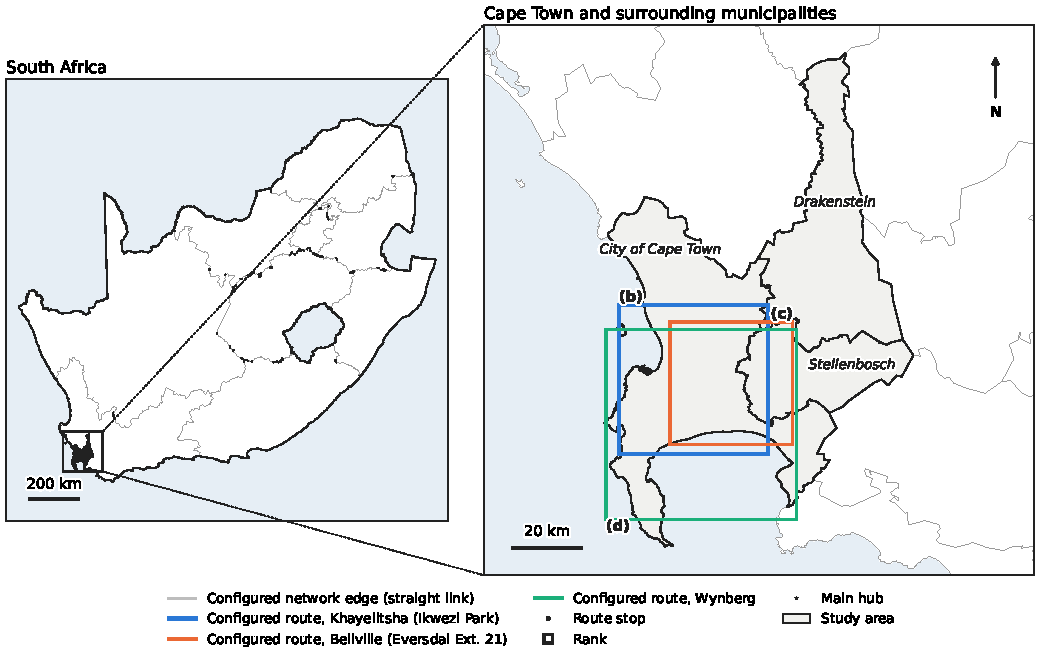
\includegraphics[width=\textwidth]{figures/fig01_study_context_a.pdf}\\[0.5em]
    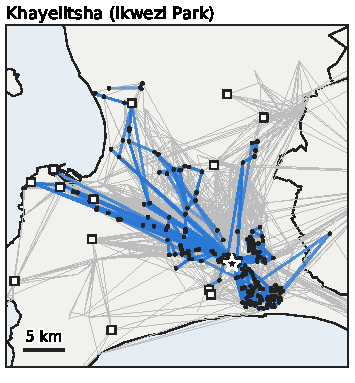
\includegraphics[width=0.32\textwidth]{figures/fig01_study_context_b.pdf}\hfill
    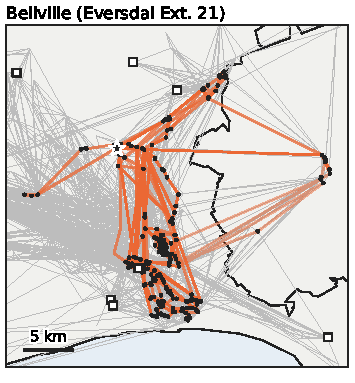
\includegraphics[width=0.32\textwidth]{figures/fig01_study_context_c.pdf}\hfill
    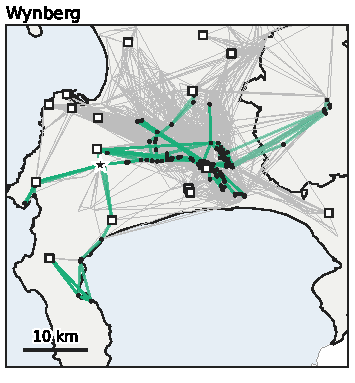
\includegraphics[width=0.32\textwidth]{figures/fig01_study_context_d.pdf}
    \caption{Study context. (a) South Africa with the study area and a zoom on Cape Town and the surrounding municipalities (Census 2011 boundaries); the coloured boxes give the extent of (b) to (d). (b) Khayelitsha, (c) Bellville and (d) Wynberg: the configured network of each community as straight links between nodes (grey), the configured routes of the community drivers as straight links between their stops (colour), the route stops (dots), the formal ranks (squares) and the main hub (star). Home nodes and the links to them are not shown.}
    \label{fig:context}
\end{figure}


% --------------------------------------------------
%   Methodology
% --------------------------------------------------

\section{Methodology}
\label{sec:methodology}

\subsection{Comparative design and shared assumptions}
\label{sec:methodology_design}

% Discuss > Establish the experimental logic before describing either model.

% Discuss > Discuss the common electrified vehicles, the fixed-mobility versus adaptive-mobility distinction, the shared charging-design space, model-native objectives, cross-evaluation and the known asymmetry in charging during rank-loading queues.
% - Assumption set abm_baseline_evidence v1 -> Higer H5C: 70.47 kWh usable, 0.38 kWh/km (about 185 km from full to empty; about 130 km in the 0.9 C to 0.2 C window), 60 kW vehicle limit, 0.90 charging efficiency.
% - The same EV values, battery window (0.2 C reserve, 0.9 C maximum), site chargers (min(P, 60 kW), first in first out) and home charging (3.7 kW, a socket outlet, at every vehicle) in both models, so differences come from the drivers. There is no case without home charging.


\begin{figure}[htb!]
    \centering
    % TODO: Redraw figures/system-diagram.drawio for the 13-step pipeline: stops -> network -> route library -> communities -> per community [routes -> fleet_scale -> demand -> baseline_config -> targets -> hand_tuning -> calibration] and [replay] -> experiments (search from the M_R design, validation, cross-evaluation, sensitivity) -> synthesis.
    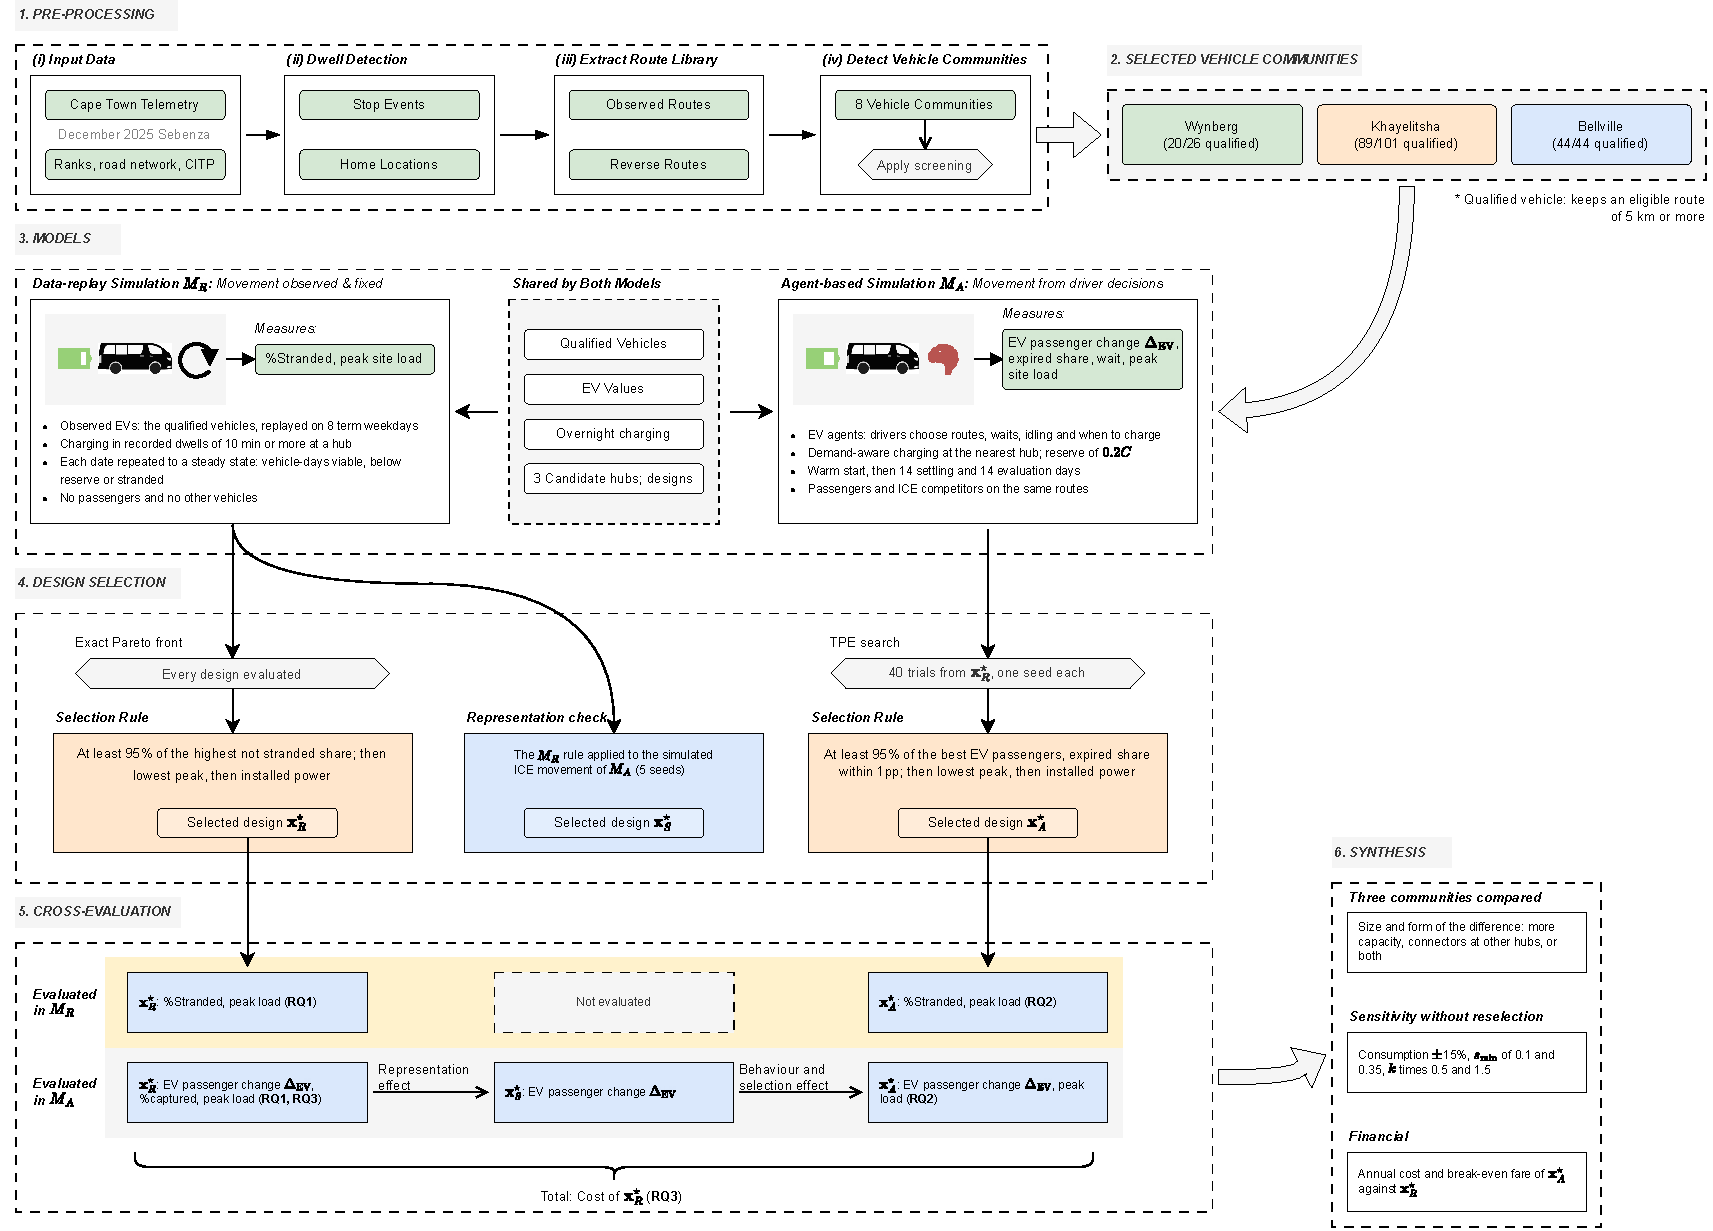
\includegraphics[width=\textwidth]{figures/system-diagram.pdf}
    \caption{
        Overview of the study design. Vehicle communities are found in the router GPS data on one Cape Town stop network, and three are selected for electrification by a frozen rule. For each community, the same observed vehicles are electrified in a data-replay model (\MR) and in an agent-based model (\MA) that also simulates synthetic internal-combustion vehicles on the community's routes. \MR{} evaluates every charging design and selects the replay design; \MA{} searches the same design space from the replay design under its own objectives. The replay design is evaluated in \MA{} beside the \MA{} design to measure the consequence of ignoring driver agency, and the results of the three communities are compared.
    }
    \label{fig:system_diagram}
\end{figure}


\subsection{Modelling minibus-taxi operations}

\subsubsection{Fixed-mobility data repplay}
% Discuss > Describe the replay of observed trajectories under electric-vehicle energy and charging constraints (Pretorius et al.), including charging queues, overnight charging, steady-state iteration and vehicle-day status classification.

\subsubsection{Decision-adaptive data replay}
% NOTE: Keep the explanation focused on the behavioural features that distinguish the adaptive model from replay and that are new from the previous Sello et al. paper.
% Discuss > Describe the event-driven simulation, driver decision mechanisms, route choice, idling, stop durations, passenger boarding, driver memory, charging decisions and evaluation horizon.

\subsubsection{Mixed-fleet population and passenger demand}

% Discuss > Explain the construction of the synthetic internal-combustion population, the population scale, the inference of passenger demand from observed departures and published boarding counts, and the assumptions used to distribute demand through the network and over time.

\subsection{Calibration and validating the agent-based model}
% Discuss > Describe the operational targets, fitting procedure, search objectives and constraints, independent-seed validation, and hold-out-day assessment. Explain which targets are essential for energy and charging analysis and which are realism checks.


\subsection{Reconstructing the operational network and vehicle communities}
\label{sec:methodology_network}

\subsubsection{Stop-event detection and network construction}

% Discuss > Describe the extraction of stop events, identification of operational nodes and directed links, treatment of formal infrastructure, and network validation.

\subsubsection{Route reconstruction and driver-specific route sets}

% Discuss > Explain the identification of anchor dwells, trip clustering, construction of representative routes and assignment of eligible routes to individual vehicles.

\subsubsection{Community detection and electrification-pilot screening}

% Discuss > Describe the multi-view similarity approach, community-detection procedure, definition of hubs, replay-based electrification screen and frozen rule used to select the three cases.


\subsection{Charging infrastructure design experiment}

\subsubsection{Candidate sites and charging-design space}

% Discuss > Define the candidate hubs, connector quantities and power levels, and the limits of the design space.

\subsubsection{Performance measures and design-selection rules}

% Discuss > Explain the reliability, passenger-service and infrastructure-load measures. Set out how each model selects a design using its own valid objectives, without implying that their objective spaces are identical.

\subsubsection{Cross-evaluation and sensitivity analysis}

% Discuss > Explain the evaluation of the replay-derived design under adaptive operation, the paired comparisons and the tested sensitivity cases.


% --------------------------------------------------
%   Results
% --------------------------------------------------

\section{Results}

\subsection{Empirical communities and model validation}

\subsection{Differences in predicted outcomes under a common design}

\subsection{Differences in selected charging infrastructure}

\subsection{Cross-model performance of the selected designs}

\subsection{Robustness and computational trade-offs}








% Discuss > The unit of analysis is a vehicle community. A pipeline of 13 named steps builds the inputs of each community: stops, network, routes (fleet library), communities, routes (driver route sets), fleet_scale, demand, baseline_config, targets, hand_tuning, calibration, replay, experiments, synthesis.

% Discuss > Each step has one settings module (each threshold with a written reason and a sensitivity check), a manifest with input, settings, code and output digests (a rerun that writes the same tables does not make the downstream steps stale), and a human decision with a diagnostic notebook. The steps have validity checks, not research gates.

% Discuss > Both models electrify the same vehicles (the community agents) with the same EV values and select from the same design space. M_R selects first; its design is the start of the M_A search and is cross-evaluated in M_A.

The study compares two representations of the same electrified vehicles. In the data-replay model (\MR), the observed movement of each vehicle is fixed, and electrification is evaluated by replaying each observed vehicle-day with the energy and charging constraints of an electric vehicle (EV)~\cite{}. In the agent-based model (\MA), movement is an output of driver decisions: drivers choose when to work, which routes to drive, how long to wait for passengers and when to charge, and they compete for passengers with the internal combustion engine (ICE) vehicles that share their corridors~\cite{}. The elements that the two models share, and the elements in which they differ, are summarised in Table~\ref{tab:model_comparison}. Movement is the treatment of the comparison, and all other elements are either identical or made equivalent, with the exception of charging during the wait in a rank loading queue, which is a known asymmetry (Section~\ref{sec:replay}).

\begin{table}[htbp]
    \centering
    \footnotesize
    \caption{Elements of the two models. Movement is the treatment of the comparison; the other elements are the same in both models, made equivalent, or present in one model only.}
    \label{tab:model_comparison}
    \begin{tabularx}{\linewidth}{@{}>{\raggedright\arraybackslash}p{0.2\linewidth}>{\raggedright\arraybackslash}X>{\raggedright\arraybackslash}Xl@{}}
        \toprule
        \textbf{Element} & \textbf{\MR} & \textbf{\MA} & \textbf{Relation} \\
        \midrule
        Electrified vehicles & The agents of the community & The same agents & Same \\
        Other vehicles & None & Synthetic ICE copies of the agents & \MA{} only \\
        Movement & Observed and fixed & Output of driver decisions & Treatment \\
        Days & The eight observed term weekdays & One typical term weekday, simulated for 14 evaluation days & Equivalent \\
        Vehicle and charging values & One assumption set & The same assumption set & Same \\
        Candidate sites and designs & The first three hubs; \((N_1, N_2, N_3, P)\) & The same & Same \\
        Overnight charging & 3.7~kW where the vehicle parks & 3.7~kW at the home node & Equivalent \\
        Charging in a rank loading queue & Yes & No & Asymmetry \\
        Passenger service & Not represented & Requests, waits and the passengers of each driver & \MA{} only \\
        Selection rule & Service near the best, then the lowest peak site load & The same principle, with a passenger measure of service & Same principle \\
        \bottomrule
    \end{tabularx}
\end{table}

The unit of analysis is a vehicle community: a group of vehicles that share hubs, routes and an operating area (Section~\ref{sec:communities}). A community is a defensible unit for an electrification pilot, because its vehicles stop at the same hubs and can therefore be served by shared chargers. A community is, however, not a taxi association, an operator or a licensed route, and the study never assigns an association to a vehicle or to a community. Three communities are selected and treated as three case studies. Since three cases do not support a statistical generalisation, RQ4 only asks whether the answers of the three communities point in the same direction.

Both models select a charging design according to the same planning principle: the selected design is the design that a planner would build, namely the design that achieves a level of service close to the best that the model can attain, at the lowest infrastructure. However, each model measures service with the outcomes that it can validly represent. \MR{} has no passengers and therefore measures service by the share of vehicle-days that are not stranded, whereas \MA{} measures service by the passengers that the EVs carry (Section~\ref{sec:objectives}). This adherence to model-native objective spaces avoids forcing a single objective space onto two models with different behavioural assumptions. \MR{} selects first, and its design is the starting point of the \MA{} search. Subsequently, the \MR{} design is evaluated in \MA{} beside the \MA{} design on the same random seeds (Section~\ref{sec:selection}), which quantifies the consequence of selecting infrastructure under the assumption of fixed mobility.

The use of the study days follows a strict separation between structural and fitted steps (Section~\ref{sec:study_days}). The structural steps, which describe where taxis stop and drive (the stop events, the network, the route library and the communities), use all 11 study weekdays, since more days provide more support. The steps that fit model inputs or driver behaviour (the fleet scale, the passenger demand, the travel times, the shifts and the calibration) use only the six calibration days, and the two hold-out days remain unseen until a calibrated model has been accepted. \MR{} has no fitted parameters and therefore replays all eight term weekdays, including the hold-out days. The school-holiday weekdays are excluded from every fit, because they represent a different demand regime.

The inputs of each community are built by a pipeline of 13 named steps, which is illustrated in Figure~\ref{fig:system_diagram}. Each step has a single settings module, in which every threshold is accompanied by a written reason and, where relevant, a sensitivity check. Each run of a step writes a manifest that records the digests of its inputs, settings, code and outputs, such that a step becomes stale only when an input, a setting or the code on which it depends has changed. Each step ends with the review of a diagnostic notebook and a recorded human decision to either accept the result or change a rule and run the step again. The steps contain implementation-validity checks (e.g., output schemas, non-empty outputs and resolvable references), but no automatic research gates. Details of the pipeline are provided in Appendix~\ref{app:reproducibility}.


\subsection{Stop events and the operational network}
\label{sec:network}
% Discuss > Stop events -> Anchored-dwell extraction; an event has 3 or more inlier points and lasts 180 s or more (from a sweep of 30 s to 600 s). Homes by the boundary-point rule (with a sensitivity table from 150 m to 1,000 m): the first and last points of 75% or more of the valid vehicle-days within 300 m of one location.

% Discuss > Nodes -> Support nodes from the two-grid method (100 m cells, 200 m complete linkage) with 5 or more stopping vehicle-days from 3 or more vehicles; formal nodes (termini, OSM ranks, railway stations, the known Site C rank) when the fleet uses them, with formal nodes within 30 m of each other merged into one; a support node within 100 m joins a formal node.

% Discuss > Passes and edges -> A pass is a straight GPS segment within 100 m of a node; it splits the movement between two stops into hops. Observed edges (2 or more vehicle-days), derived reverse edges and close-node links (300 m), all with OSM road lengths.

% Discuss > Review and coverage -> One review of 211 items (2 of 30 candidate cells, 153 of 168 edges and all 13 conflicts accepted). 726 nodes (18 ranks), 98.9% in the largest strongly connected component; 76% of the stop events and 72% of the dwell captured; 66.5% of the distance between stops represented. Details in Appendix~\ref{app:network}.

Stop events are extracted from the GPS trajectories with an anchored-dwell algorithm that tolerates isolated positioning errors. A candidate stop is anchored at the median position of its first three inlier points, and a later point is an inlier when it lies within 30~m of the anchor and the pairwise diameter of the inliers remains at or below 60~m. One isolated outlier is permitted when the subsequent point returns to the candidate, whereas a second consecutive outlier, or a reporting gap of more than 300~s, ends the candidate. A candidate becomes a stop event when it contains at least three inlier points, has an outlier share of at most 10\%, and lasts at least \( T_{\min} = 180 \)~s, a value that was selected from a sweep of 30 to 600~s. At the sampling interval of about 80~s, three inlier points span at least about 160~s. Consequently, stops shorter than about 2 to 3 minutes, which include most of the boarding and alighting stops along a route, cannot be observed in the data. The location of a stop event is the median of its inlier positions.

The home base of each vehicle is identified with a boundary-point rule. The first and last points of each valid vehicle-day are collected, the boundary point with the most other boundary points within \( R_{\text{home}} = 300 \)~m is selected as the candidate, and the home location is the median of the boundary points within \( R_{\text{home}} \) of the candidate. A vehicle has a home when both the first and the last points of at least 75\% of its valid vehicle-days lie within \( R_{\text{home}} \) of this location; otherwise, its most frequent first point is used as its start location. The sensitivity of the rule was assessed for radii from 150 to 1{,}000~m and minimum shares of 0.6, 0.75 and 0.9.

A single operational network is constructed for the whole study area and is used by all communities. Rather than representing the full road network, the network represents the locations at which taxis stop in an operationally important way, the fixed infrastructure that the fleet uses, and the links between these locations, such that nodes are derived from evidence of stopping and edges from evidence of driving. The eligible stop events (inside the study area, on valid weekday vehicle-days, and not at a home unless that home is at infrastructure) are counted in two square grids of 100~m cells with offsets of 0 and 50~m, so that a rank on a cell boundary is not split into two weakly supported cells. A cell is selected when it contains stop events from at least \( N_{vd} = 5 \) vehicle-days and \( N_v = 3 \) distinct vehicles. This support rule replaces the classifier of an earlier stop-network method and achieved a higher precision and F1 score than the classifier on held-out labelled cells from Gauteng. The selected cells are merged into support nodes by connected complete-linkage clustering with a maximum diameter of \( D_{\max} = 200 \)~m, which prevents long spatial chains, and each stop event is associated with one node only.

Formal nodes are obtained from the City of Cape Town minibus-taxi route termini, the taxi ranks and railway stations in OpenStreetMap (OSM), and one large rank that these sources omit, namely the Site C rank in Khayelitsha, which was confirmed on satellite imagery (Section~\ref{sec:spatial_data}). Formal nodes within 30~m of each other are merged into one node, a formal node is retained only when the fleet stops there, and a support node within the snap distance \( S = 100 \)~m of a formal node joins it and adopts its location. Home bases that are not at infrastructure become home nodes, which vehicles can reach but cannot traverse.

Since a moving vehicle covers a median distance of 435~m between consecutive GPS points, a vehicle can pass through several nodes between two stop events without a detected stop. A pass is therefore recorded when the straight line between two consecutive GPS points comes within \( r_{\text{pass}} = 100 \)~m of a node, with the pass time and cumulative distance interpolated at the point of closest approach. Passes split the movement between two stop events into hops, but they do not count towards the support of a node, so that nodes remain defined by where taxis stop. The network contains three kinds of directed edges: observed edges, which join the two nodes of a hop and are retained when at least two vehicle-days use them; derived reverse edges for observed edges without an observed counterpart; and close-node links in both directions between nodes within \( D_c = 300 \)~m of each other, which allow short movements between nearby nodes without long detours. All edge lengths are shortest road paths on the drivable OSM network, such that one-way streets are respected.

Rather than relying solely on automatic rules, the network is subjected to a single manual review of 211 items, which comprise candidate cells with high vehicle-day support but few vehicles, edges with implausible ratios of road length to straight-line length or implausible speeds, and conflicts between support nodes and formal nodes. Each item was reviewed in an interactive map that plays back the relevant vehicle-days, and 2 of 30 candidate cells, 153 of 168 flagged edges and all 13 conflicts were accepted. The resulting network comprises 726 nodes, of which 18 are ranks, and 98.9\% of the nodes lie in the largest strongly connected component. The nodes capture 76\% of the eligible stop events and 72\% of their dwell time, and 66.5\% of the distance driven between stop events runs on network edges. The parameter sweeps and coverage measures are presented in Appendix~\ref{app:network}.

\subsection{Route library and driver route sets}
\label{sec:routes}
% Discuss > Trips -> A trip runs between two anchor dwells (600 s or more at a non-home node); a trip back to the same terminal is a loop. Route stops are all visited nodes, stops and passes.
% Discuss > Variants -> Trips of a terminal pair are clustered by the Jaccard similarity of their node sets (0.5); the representative is the medoid, and a pass stays when half or more of the cluster's trips visit it. A variant qualifies with trips on 3 or more vehicle-days and 2 or more dates.
% Discuss > Library and route sets -> One fleet library: 586 routes and 503 derived reverse routes. Each driver's eligible routes are the smallest set that covers 80% of its trip distance on qualified routes, with their reverse counterparts and the two halves of each loop; routes shorter than 5 km in the network are left out.
% Discuss > Limit -> A route is one unit in M_A: a driver cannot charge at a rank inside a route, so an EV does not select a route that it cannot finish from a full battery.

Minibus taxis typically operate in a fill-and-go manner, in which a vehicle loads passengers at a terminal and departs when it is full~\cite{woolf2013_people_centred_paratransit,behrens2016_paratransit_african_cities}. Long dwells at network nodes therefore mark the terminals of operation. An anchor dwell is defined as a stop event of 600~s or more at a node that is not a home, and a trip runs from the end of one anchor dwell to the start of the next anchor dwell in the same vehicle-day. The node sequence of a trip contains its origin, its intermediate stop nodes and passes in time order, and its destination, and a trip that returns to its origin is a loop.

Since the intermediate nodes of a taxi vary from trip to trip between the same terminals, the observed trips are compressed into representative routes. For each ordered terminal pair, the distinct node sequences are processed in order of decreasing support, and a sequence joins the most similar existing variant when the Jaccard similarity of their node sets~\cite{jaccard1912_flora_distribution} is at least \( \theta = 0.5 \); otherwise, it founds a new variant. A variant qualifies as a route when its trips occur on at least three vehicle-days and two dates. The representative of a qualifying variant is its medoid, i.e., the observed trip with the highest mean similarity to the other trips of the variant, and the stops of the route are the terminals and stop nodes of the medoid, together with each pass that at least half of the variant's trips visit. This majority rule removes the noise of parallel roads while retaining the nodes at which taxis consistently search for passengers. All route nodes are possible stops, and whether a driver stops at a node is a behavioural decision in \MA{} (Section~\ref{sec:abm}).

The route library is built from the trips of the whole fleet, because a corridor is a property of the operation and more vehicles provide more support. Each route receives a reverse counterpart, which is either the most similar qualified route in the opposite direction or a derived route with the reversed node sequence. Additionally, each loop is split at its turning node (the node farthest from the origin) into an outward and a return half, so that a taxi can turn at the turning node and start a new run there. The resulting library comprises 586 qualified routes and 503 derived reverse routes.

The eligible routes of a driver are the smallest set of its routes, ordered by their share of its trip distance on qualified routes, that covers 80\% of that distance, together with the reverse counterparts of these routes and the two halves of each eligible loop. In the selected communities, routes shorter than 5~km in the network are excluded, since a route whose node sequence retains only a few nodes can be much shorter in the network than its observed trips and would cause an agent to drive too little. A vehicle with at least one eligible route becomes an agent of both models. The routes carry no time of day, and the direction and timing of demand are instead handled by the demand model (Section~\ref{sec:demand}). Finally, a route is treated as a single unit of operation in \MA: once a driver has started a route, it cannot charge at a rank along that route. Consequently, an EV does not select a route that it cannot complete from a full battery (Section~\ref{sec:abm}).

\subsection{Vehicle communities and pilot selection}
\label{sec:communities}
% Discuss > Partition -> Four TF-IDF views per vehicle (dwell nodes, network edges, formal ranks, pairs of consecutive anchor dwells of 600 s or more); mean cosine similarity over shared views; 15-nearest-neighbour graph; Leiden with a resolution sweep, 50 seeds and a consensus partition. A resolution is eligible when 90% or more of corridor use stays inside one community; the most stable eligible resolution is chosen (0.75, 8 communities). Evidence tests in Appendix~\ref{app:communities}.
% Discuss > Hubs -> Non-home nodes ranked by the number of distinct community vehicles that dwell there for 20 min or more. The same rule gives the candidate charging sites.
% Discuss > Electrification screening -> The M_R EV core replays each valid vehicle-day under three scenarios: overnight charging only (V1), overnight plus 60 kW at the first three hubs (V2), and hubs only (V3). Overnight charging uses the time between the driving windows of consecutive days. No connector limit.
% Discuss > Frozen selection rule -> 15 or more vehicles; formal main hub; hub charging binding (V2 - V1 >= 15 percentage points); median driver with 30% or more of its trip distance on its eligible routes; distinct main hubs. No minimum of V2. Rank by V2 and select three.
% Discuss > Names -> From the Census main places of the hub and its main partner place: Khayelitsha (Ikwezi Park), Bellville (Eversdal Ext. 21) and Wynberg.

Vehicle communities are detected with a multi-view similarity graph. Each vehicle is described by four views of non-negative feature weights, which are computed from the stop events and edges inside the study area on valid weekdays: the dwell hours at each non-home node, the vehicle-days on each network edge, the dwell hours at each formal node, and the vehicle-days with each pair of consecutive anchor dwells (origin-destination pairs). The features of each view are weighted with term frequency-inverse document frequency (TF-IDF)~\cite{salton1988_term_weighting}:
\begin{equation}
    \tilde{x}^{(m)}_{vf} = \ln\left(1 + x^{(m)}_{vf}\right)\left(\ln\frac{1 + n}{1 + \mathrm{df}_f} + 1\right),
\end{equation}

\noindent where \( x^{(m)}_{vf} \) is the weight of feature \( f \) for vehicle \( v \) in view \( m \), \( n \) is the number of vehicles, and \( \mathrm{df}_f \) is the number of vehicles that use feature \( f \). Each weight vector is subsequently normalised to unit length, such that a hub used by the whole fleet contributes less to the similarity of two vehicles than a stop shared by only a few. The combined similarity \( S_{uv} \in [0, 1] \) of vehicles \( u \) and \( v \) is the mean cosine similarity over the views that both vehicles have. A similarity graph joins each vehicle to its 15 most similar vehicles, and the Leiden algorithm~\cite{traag2019_louvain_to_leiden} partitions the graph by maximising the modularity with a resolution parameter \( \gamma \)~\cite{newman2004_community_structure,reichardt2006_statistical_mechanics_communities}:
\begin{equation}
    Q_\gamma = \frac{1}{2W} \sum_{u,v} \left[ A_{uv} - \gamma \frac{k_u k_v}{2W} \right] \mathbf{1}\left[c_u = c_v\right],
\end{equation}

\noindent where \( A_{uv} \) is the edge weight between vehicles \( u \) and \( v \), \( k_u \) is the strength of vehicle \( u \), \( W \) is the total edge weight, \( c_u \) is the community of \( u \), and \( \mathbf{1}[\cdot] \) is the indicator function. A larger \( \gamma \) produces smaller communities.

For each resolution \( \gamma \in \{0.25, 0.5, 0.75, 1, 1.25, 1.5, 2, 2.5, 3\} \), the Leiden algorithm is run with 50 seeds, and the seed partitions are combined into a consensus partition~\cite{lancichinetti2012_consensus_clustering}. A resolution is eligible when its median seed partition contains at least two communities of five or more vehicles, and when its consensus partition retains at least 90\% of corridor use within one community, where a corridor is an undirected pair of consecutive anchor dwells that recurs on at least three vehicle-days and two dates. The latter condition encodes the operational meaning of a community, namely vehicles that share corridors in a common operating area. Of the eligible resolutions, the most stable resolution, as measured by the mean pairwise adjusted Rand index (ARI)~\cite{hubert1985_comparing_partitions} of its seed partitions, is selected. Vehicles in communities of fewer than five vehicles are not assigned to a community. The existence of the communities is tested against a null model of randomised fleets~\cite{strona2014_curveball}, and their seed stability, temporal stability and agreement across views are assessed in Appendix~\ref{app:communities}.

The hubs of a community are its non-home nodes, ranked by the number of distinct community vehicles that dwell there for 20~min or more, and the first-ranked hub is the main hub. The first three hubs are the candidate charging sites of both models, which ensures that the screening and the design evaluation cannot disagree on where chargers may be placed.

Each community is screened for electrification by replaying its valid vehicle-days, excluding long-distance days, with the energy core of \MR{} (Section~\ref{sec:replay}) and the vehicle values of Section~\ref{sec:vehicle_assumptions}, under three scenarios: overnight charging only, overnight charging combined with charging at the first three hubs, and hub charging only. The viable shares \( V_1 \), \( V_2 \) and \( V_3 \) denote the shares of the screened vehicle-days that are viable in each scenario, where a vehicle-day is viable when its lowest battery level remains at or above the reserve of \( 0.2\,C \), with \( C \) the usable battery capacity. A hub charging opportunity is a stop of 20~min or more at a candidate hub, at which a vehicle that arrives below \( 0.6\,C \) charges at 60~kW up to \( 0.9\,C \), without a limit on the number of connectors. Overnight charging at 3.7~kW is applied over the parked time between the driving windows of consecutive days (Section~\ref{sec:replay}). The sessions of the second scenario also provide the connector estimate \( \hat{N}_j \) of each candidate hub, which is defined as the 95th percentile of the daily peak number of simultaneous sessions, rounded up, and which bounds the design space (Section~\ref{sec:objectives}).

A community is a candidate pilot when it satisfies four conditions. First, it has at least 15 vehicles. Second, its main hub is formal (a rank, a station or a terminus), so that chargers would stand at real infrastructure. Third, hub charging is binding, i.e., \( V_2 - V_1 \geq 15 \) percentage points, since the charger design is irrelevant when overnight charging alone is sufficient, in which case the comparison of the two models has nothing to test. Fourth, its median driver has at least 30\% of its trip distance on its eligible routes, so that the \MA{} agents can drive most of their observed operation. The candidates are ranked by \( V_2 \), and the first three candidates with distinct main hubs are selected. No minimum is imposed on \( V_2 \), because the long daily distances of the fleet leave many observed days unviable even with unlimited chargers at three hubs. The rule was frozen before any agent-based simulation was run. Since the rule selects on the screening outcome, the results apply to communities that are suitable for an electrification pilot. The selected communities are named after the Census main places of their main hub and its main partner place: Khayelitsha (Ikwezi Park), Bellville (Eversdal Ext.~21) and Wynberg.

\subsection{Data replay model}
\label{sec:replay}
% Discuss > Principle -> M_R replays the observed movement of each community agent with the EV physics; movement, timing and dwells are fixed, and a vehicle cannot drive to a charger. --- Pretorius et al. 2022, Booysen et al. 2023, Booysen et al. 2026.
% Discuss > Steady state -> Each replayed date starts at 0.9 C and repeats to its own steady state (tolerance 0.001 C). Vehicle-days with a charging opportunity at a candidate site iterate together, because they share the connectors.
% Discuss > Charging -> A site opportunity is a stop event of 10 min or more within 100 m of a site with connectors; a vehicle below 0.9 C joins a first-in, first-out queue and charges until 0.9 C or its observed departure. Overnight charging at 3.7 kW over the time between the driving windows. M_R charges during the wait in the rank loading queue, so it is optimistic on this point.
% Discuss > Day status -> viable, below_reserve (lowest level between 0 and 0.2 C), stranded (at or below 0) or non_converged.

\MR{} follows the trajectory-replay approach of earlier minibus-taxi electrification studies~\cite{pretorius2024_grid_mobility_interdependence,pretorius2025_viability_minibus_taxi_evs,booysen2026_cpt_embt_transition}, in which the observed movement of each vehicle is replayed with the physics of an EV~\cite{pearre2011_ev_range_requirements}. The movement, timing and dwell locations of each vehicle are fixed, and the replay replaces the fuel use of each observed vehicle-day with the energy use of the study EV, without changing its routes, departures, dwells or passengers. For each charging design, \MR{} therefore answers a single question: can each observed vehicle-day be driven by the EV with the chargers of the design? Importantly, a vehicle charges only when it is parked near a charger for long enough, and it cannot drive to a charger. The replayed vehicles are the agents of the community, such that both models electrify the same vehicles, and the replayed days are their valid vehicle-days on the eight term weekdays, excluding long-distance days. Since the energy of a driven distance \( \Delta s \) is \( e\,\Delta s \), where \( e \) is the energy intensity, the replay requires only the cumulative distance of each vehicle at the start and end of each stop event rather than the GPS points.

A charging opportunity is a stop event of 10~min or more within 100~m of a site with connectors. All vehicle-days of a date are replayed in one chronological sequence, so that the vehicles share the connectors. At the start of an opportunity, a vehicle below \( 0.9\,C \) joins the first-in, first-out queue of the site. A free connector is assigned to the first vehicle in the queue, and the session adds the battery power \( \eta \min(P, P_v) \) until the vehicle reaches \( 0.9\,C \) or its observed stop ends, where \( P \) is the connector power, \( P_v \) is the vehicle charging limit and \( \eta \) is the charging efficiency. A vehicle always departs at its observed time, and a vehicle that is still queued at that time does not charge. Since a vehicle that cannot drive to a charger later must take every opportunity to charge, the trigger level is equal to the charge limit. The dwell at a rank includes the wait in the loading queue, and \MR{} therefore charges during this wait whenever a connector is free, which implicitly assumes connectors at the loading bays. In this respect, \MR{} is optimistic relative to \MA, in which a driver must leave the rank to charge.

Every vehicle additionally charges overnight at \( P_o = 3.7 \)~kW where it parks. Since the routers continue to report while a vehicle is parked, the overnight period is derived from the driving window of each vehicle-day, which starts at the end of the stop event that contains the first point of the day and ends at the start of the stop event that contains the last point. The overnight energy is given as follows:
\begin{equation}
    E^{\text{night}} = \min\left(0.9\,C - E^{\text{end}},\ \eta \min(P_o, P_v)\, \Delta t_{\text{park}}\right), \qquad \Delta t_{\text{park}} = t^{\text{start}} + 24\,\text{h} - t^{\text{end}},
\end{equation}

\noindent where \( E^{\text{end}} \) is the battery energy at the end of driving, and \( t^{\text{start}} \) and \( t^{\text{end}} \) are the start and end of the driving window.

A single replay of a date from a full battery does not show whether a vehicle can sustainably repeat that day. Following~\cite{booysen2026_cpt_embt_transition}, each date \( d \) is therefore iterated to a steady state:
\begin{equation}
    \mathbf{s}^{(0)} = 0.9\,C\,\mathbf{1}, \qquad \mathbf{s}^{(i+1)} = \Phi_d\left(\mathbf{s}^{(i)};\, A^{(i)}\right),
\end{equation}

\noindent where \( \mathbf{s}^{(i)} \) is the vector of start levels of the active vehicle-days \( A^{(i)} \) in iteration \( i \), and \( \Phi_d \) is one chronological replay of the date followed by the overnight charging. A vehicle whose battery level falls to zero strands and leaves the active set, whereas a vehicle below the reserve but above zero continues its observed day. The iteration terminates at a fixed point (the same active set and a maximum change in start levels of at most \( 0.001\,C \)), at a sustainable cycle (a start vector within \( 0.001\,C \) of one of the last ten start vectors), when no active vehicle remains, or after 100 iterations without convergence. Only the vehicle-days with a charging opportunity at a candidate site share connectors and iterate together, whereas all other vehicle-days are independent of the design and are computed once.

Each replayed vehicle-day is assigned one of four statuses: viable (a lowest level of at least \( 0.2\,C \)), below reserve (a lowest level between zero and \( 0.2\,C \)), stranded (a level at or below zero) or not converged. A day below the reserve would require a change of the observed operation, which \MR{} cannot represent, whereas a stranded day cannot be driven at all. Since stranding is also the failure mode of \MA, the stranded share is the like-for-like reliability measure of the comparison.

\subsection{Agent-based model}
\label{sec:abm}
% Discuss > Engine -> parasim-engine (Sello et al.), event-driven; described by the ODD protocol in Appendix~\ref{app:abm}. Drivers decide when to work, which route to drive (utility with a temperature), how long to wait at a stop (soft demand-aware stop rule, with the remembered demand of the route being driven in the current interval of the day; first stop at the rank) and when to idle; drivers learn route and demand memories. --- Mention the changes against the earlier model.
% Discuss > Population -> The community agents (observed vehicles) and seeded ICE copies: each agent gets floor or ceiling of k - 1 copies, so the population is k times the agents (Khayelitsha 1,358, Bellville 1,673, Wynberg 686 drivers). A copy takes the routes, idle locations and shifts of its agent; its home is one of the 5 nearest nodes, and its shift moves by a normal draw (30 min). State the representativeness assumption.
% Discuss > Network and time -> Windowed log-normal travel times from the observed hops of the calibration days; hops slower than 5 km/h hold a stand and are left out of the fit; in Khayelitsha the log-normal excess is scaled by a factor for each time window. Engine ranks are the formal ranks. Shifts from the first and last movement of each calendar day of the calibration days.
% Discuss > Horizon -> A measured warm-up (49 to 91 days; the first day after which the 7-day mean of each measure stays within 2% of its long-run mean on 3 seeds), kept as a warm start of the driver memories; each run then has 14 settling days and 14 evaluation days.
% Discuss > Electric vehicles -> The agents are EVs and the copies stay ICE. demand_aware charging policy (0.2 C and 0.9 C); a driver charges only off a route, at the nearest station, and waits in its queue. Reserve rules: no route start without the energy for the route, the drive to a station and the 0.2 C reserve; no drive home below the reserve; no route that a full battery cannot finish. A driver at a station takes a connector only when its policy says charge and its shift has not ended, or when its energy is below the need of its cheapest route; the energy of the last charging step counts. A stranded EV restarts at home with a full battery. State that these engine corrections replace the earlier behaviour and do not change the ICE runs.

\MA{} is implemented in parasim-engine, the event-driven discrete-event simulation framework of~\cite{sello2025_stellenbosch_embt_abm}, in which the minibus taxis of a community are represented as driver agents that decide when to work, which route to drive, how long to wait at a stop, when to idle and, in the case of an EV, when to charge. Passenger requests are generated from the latent demand of Section~\ref{sec:demand}, and movement is therefore an output of the model. Every simulated day represents the same typical term weekday, time is continuous, and space is the operational network of Section~\ref{sec:network}. The model is described in full according to the overview, design concepts and details (ODD) protocol~\cite{grimm2020_odd_protocol} in Appendix~\ref{app:abm}, and this section summarises the mechanisms that are relevant to the comparison. Relative to the framework of~\cite{sello2025_stellenbosch_embt_abm}, the stop rule now uses a route-specific memory of demand, the first stop of a route represents loading at the rank with its own parameters, an optional last-run rule limits late-night operation, and revised charging rules prevent drivers from starting routes that they cannot complete.

\paragraph{Drivers and population}
The drivers of a community comprise its agents and their synthetic ICE copies. Each agent keeps its home node, its eligible routes and its idle locations, which are the terminals of its routes. Since the observed vehicles are only a sample of the taxis that operate from a hub, each agent receives \( \lfloor k - 1 \rfloor \) or \( \lceil k - 1 \rceil \) ICE copies from a seeded Bernoulli draw, such that the population is on average \( k \) times the number of agents, where \( k \) is the scale factor of Section~\ref{sec:demand}. A copy adopts the routes, idle locations and shift pattern of its agent, its home is drawn from the five network nodes nearest to the agent's home, and the start and end of its shift are moved by a common normal draw with a standard deviation of 30~min. This construction rests on the assumption that the observed agents are representative of the taxis that load at the hub of the community, both in the routes that they drive and in their working hours. The resulting populations comprise 1{,}358, 1{,}673 and 686 drivers in Khayelitsha, Bellville and Wynberg, respectively, of which the electrified agents form only 2.6\% to 6.6\% (Table~\ref{tab:models}).

Each agent has a typical-weekday shift, of which the start and end times are normally distributed with the mean and standard deviation of the first and last movements on its calendar days in the calibration period, and each day is a working day with the observed probability of activity. Two calibrated parameters, the shift spread \( \psi \) and the shift end offset \( \delta \), scale the standard deviations and move the mean end time, respectively. The offset is necessary because the observed end of a shift is the arrival at home, whereas the simulated end is the time at which the driver starts to return home. In Khayelitsha, a last-run rule additionally prevents a driver from starting a route that it expects to end after its shift end, because too many agents otherwise remained active late at night.

\paragraph{Network and travel time}
The travel time of an edge \( \ell \) that a driver enters in time window \( w \) is modelled as follows:
\begin{equation}
    T_\ell = \frac{s_\ell}{80\ \text{km/h}} + X_{\ell w}, \qquad
    X_{\ell w} =
    \begin{cases}
        0, & \text{with probability } \pi_{\ell w}, \\
        c_w Y, \quad \ln Y \sim \mathcal{N}\left(\mu_{\ell w}, \sigma_{\ell w}^2\right), & \text{otherwise},
    \end{cases}
\end{equation}

\noindent where \( s_\ell \) is the road length of the edge, \( \pi_{\ell w} \) is the share of observed hops without excess time, \( \mu_{\ell w} \) and \( \sigma_{\ell w} \) are the parameters of a log-normal fit of the observed excess times~\cite{fosgerau2012_travel_time_variability}, and \( c_w \) is an optional excess factor. The four time windows are the night (19:00 to 06:00), the AM peak (06:00 to 09:00), the midday (09:00 to 15:00) and the PM peak (15:00 to 19:00). The fit uses the hops of the whole fleet on the calibration days, excluding hops slower than 5~km/h, since such hops contain a stand rather than driving and would make the simulated vehicles much slower than the observed vehicles. Edges with fewer than five retained hops receive a fixed excess from the pooled speed of the window, reverse edges copy the model of their observed counterpart, and close-node links use the median speed of the short observed edges. In Khayelitsha, where the simulated agents drove faster than the observed vehicles in every window, the excess is scaled by a factor \( c_w \) for each window to match the observed median speed. Drivers travel along shortest paths by road length~\cite{dijkstra1959_note_on_two_problems}, and the model does not represent congestion. Only the 18 formal ranks of the network act as engine ranks with loading queues.

\paragraph{Decisions}
A driver that is not on a route first returns home when its shift has ended. Otherwise, an EV driver consults its charging policy, after which the driver chooses between its routes and idling with a multinomial logit model~\cite{mcfadden1974_conditional_logit,train2009_discrete_choice}:
\begin{equation}
    \Pr(j) = \frac{\exp\left(U_j / \tau(t)\right)}{\sum_{i} \exp\left(U_i / \tau(t)\right)},
\end{equation}

\noindent where \( U_j \) is the utility of route \( j \) or of idling, and \( \tau(t) \) is a temperature that decreases from 1 to 0.1 during an initial exploration period of ten days, such that drivers initially sample all of their routes~\cite{sutton2018_reinforcement_learning}. The utility of a route is a weighted sum of normalised features: the waiting requests at the current node that the route can carry, the competing drivers at the node on the same route, and the remembered distance, passengers and passenger distance per run of the route in the current interval of the day. The utility of idling comprises a bias \( \beta_0 \), a demand term with weight \( \beta_h \) that increases as the driver's remembered demand in the current interval decreases, and a small income term, such that drivers idle more during intervals that they remember as quiet. The route weights are fixed at the values of an earlier calibration of the model, whereas \( \beta_0 \) and \( \beta_h \) are calibrated (Section~\ref{sec:calibration}).

When a driver arrives at a stop, its passengers for that stop alight, compatible waiting requests board, and the driver joins the loading queue if the node is a rank. The driver then keeps waiting with probability
\begin{equation}
    \pi = \left[ 1 + \exp\left(-\left(b + w_d\, d - w_o\, o\right)\right) \right]^{-1}, \qquad
    d = \min\left(\frac{\bar{m}_{r,t}}{Q},\ 1\right), \qquad
    o = \frac{m_{\text{on}}}{Q},
\end{equation}

\noindent where \( \bar{m}_{r,t} \) is the driver's remembered number of passengers per run of route \( r \) in the current interval \( t \), \( m_{\text{on}} \) is the number of passengers on board, \( Q = 15 \) is the number of seats, and \( b \), \( w_d \) and \( w_o \) are the bias, the demand weight and the occupancy weight. Without a memory of the route in the interval, \( d \) is drawn uniformly, so that drivers explore until their memory fills. The decision is re-evaluated at exponentially distributed intervals with a mean of 60~s, and the stop ends after a maximum duration \( T_{\max} \). The first stop of a route represents fill-and-go loading at the rank and therefore has its own bias, demand weight and maximum duration, such that a driver waits to fill where it remembers demand and departs promptly where it does not.

A passenger boards only a taxi that is at the origin node, has a free seat and serves a route on which the destination follows the origin; at a rank, the first compatible taxi in the loading queue is selected. Otherwise, the request waits and expires after 2~h. Passengers do not walk to other nodes or switch to other modes. The memory of each driver records the distance, duration, passengers and passenger distance of each completed route run, as well as the queue length, waiting time and charging time of each charging visit, as streaming statistics in 30-minute intervals of the day. A driver therefore learns where and when its routes carry passengers.

\paragraph{Initialisation and run horizon}
A cold run starts with empty memories and runs a warm-up period followed by 14 evaluation days~\cite{welch1983_statistical_analysis_simulation,law2015_simulation_modeling}. The warm-up length of each community, between 49 and 91 days, is the first day after which the seven-day means of the served passengers, their share of the requests, the occupancy and the route-choice shares remain within a tolerance of their long-run means on three seeds, rounded up to whole weeks. To reduce the computational cost, the warm-up is run once, and the resulting driver memories are saved as a warm start. Each subsequent run loads these memories, disables exploration, and runs 14 settling days followed by 14 evaluation days.

\paragraph{Electric vehicles and charging}
In the electrification experiments, the agents become EVs with the vehicle and charging values of \MR{} (Section~\ref{sec:vehicle_assumptions}), whereas the copies remain ICE vehicles. An EV driver charges according to a demand-aware policy: it always charges below \( s_{\min} = 0.2 \), never charges above \( s_{\max} = 0.9 \), and charges between these levels when
\begin{equation}
    \frac{E(t)}{C} < s_{\min} + \left(s_{\max} - s_{\min}\right)\left(1 - \hat{h}_t\right),
\end{equation}

\noindent where \( E(t) \) is the battery energy and \( \hat{h}_t \in [0, 1] \) is the driver's normalised remembered demand in the current interval. A driver therefore charges more readily during quiet periods, which reflects the opportunity cost of charging during busy periods. A driver decides to charge only when it is not on a route, and it charges at the nearest station, where it waits in a first-in, first-out queue. In contrast to \MR, a driver in a rank loading queue therefore cannot charge without leaving the rank.

To prevent avoidable stranding, an EV maintains a reserve of \( 0.2\,C \). It does not select a route that a full battery cannot complete together with the drive from the last stop to the nearest station and the reserve. Moreover, it starts a route only when its energy covers the drive to the first stop, the route, the drive to the nearest station and the reserve, and otherwise charges first, and it charges before returning home when it would otherwise arrive below the reserve. At a station, a driver takes a connector only while it still needs to charge: before its shift end, while it is below its charge target or the energy needed for its cheapest route, or while its policy requests charging; and after its shift end, only while it would otherwise arrive home below the reserve. Home charging at 3.7~kW is applied for the time at home. An EV that nevertheless strands loses the passengers on board and is restored at home with a full battery at the next day start. These rules are corrections of the engine that replace its earlier charging behaviour without a setting to revert to it. Since ICE drivers never charge, the corrections do not change the ICE runs, which was verified by reproducing the logs of a frozen ICE run exactly.

\subsection{Corridor population and passenger demand}
\label{sec:demand}
% Discuss > Departures and load factors -> A departure is an anchor-to-anchor trip of 1 km or more that leaves the origin catchment. Its load factor is 1, except in the counter-peak direction of the AM and PM peaks, where it is the counter-peak to peak ratio of CITP Table 3-18 (mean 0.21 without a survey). Peak direction from the survey, else from the residential end (OSM land use).
% Discuss > Scale factor k -> k = facility boardings at the main hub / (15 seats x the summed load factors of the agents' departures from the hub per calibration day), with the departures moved onto the agents' eligible routes. Khayelitsha 15.21, Bellville 38.03, Wynberg 34.3 (after the removal of routes shorter than 5 km, which left fewer agents). The register gives an upper bound; the Bellville k is above it.
% Discuss > Demand -> Rank loading: a share alpha = 0.8 (a judgement value) of the passengers boards at the origin terminal and alights along the route; the rest board and alight between en-route nodes. Only servable OD pairs get demand. Daily level k x sum of 15 lambda / alpha over the departures, so the terminal requests at the hub equal the facility boardings.
% Discuss > Timing -> One typical weekday; Wynberg by the observed departures and trips home, Khayelitsha and Bellville by the observed moving time moved to the boarding time. Requests are Poisson counts and expire after 2 h.

Since passenger demand cannot be observed in GPS data, an effective latent demand is inferred for the modelled taxis. The observed departures, routes and stops of the agents provide its structure, direction and timing, whereas published facility boarding counts set its level through the scale factor \( k \). The demand follows rank loading: most passengers board at the rank, the taxi departs when full, and the passengers alight along the route, while fewer passengers board along the way~\cite{woolf2013_people_centred_paratransit,behrens2016_paratransit_african_cities}.

A departure is an anchor-to-anchor trip of an agent on the calibration days that is at least 1~km long and leaves the catchment of its origin. The catchment is defined as all nodes within 300~m of the same facility of the Comprehensive Integrated Transport Plan (CITP) of the City of Cape Town or, if no such facility exists, the origin node alone, which removes short movements within a rank complex. Since the stop rates, slow-moving shares and speeds of the observed trips do not distinguish loaded from empty legs at this sampling interval, the direction of demand is taken from survey data. Each departure receives a load factor \( \lambda \), which equals 1 except for departures in the counter-peak direction of a corridor during the AM peak (06:00 to 09:00) and in the AM-peak direction during the PM peak (15:00 to 19:00). For these departures, \( \lambda \) equals the ratio of counter-peak to peak vehicle trips on the corridor in CITP Table 3-18, which ranges between 0.09 and 0.39, or the mean ratio of 0.21 for corridors without a survey. The peak direction of a corridor is the surveyed direction with more AM-peak trips or, for corridors without a survey, the direction from its residential end, which is identified from OSM land use. Since the agents drive only their eligible routes in \MA, the departures of each agent are moreover redistributed onto its eligible routes in proportion to their load factors with a weight \( \omega_d \), such that each agent retains its total load and the supply and demand remain consistent with what the agents drive.

The scale factor is the ratio of the full population of taxis that load at the main hub to the agents:
\begin{equation}
    k = \frac{B}{Q\,L}, \qquad L = f \sum_{d \in \mathcal{H}} \lambda_d\, \omega_d, \qquad f = \frac{n_{\text{active}}}{n_{\text{valid}}\,\lvert \mathcal{D}_c \rvert},
\end{equation}

\noindent where \( B \) is the daily number of boardings at the CITP facility of the main hub (Section~\ref{sec:spatial_data}), \( \mathcal{H} \) is the set of agent departures from the hub catchment on valid vehicle-days, and \( L \) is the number of full loads of the agents per day. The day factor \( f \) converts counts on valid vehicle-days to counts per calibration day, where \( n_{\text{active}} \) and \( n_{\text{valid}} \) are the active and valid agent vehicle-days and \( \lvert \mathcal{D}_c \rvert = 6 \) is the number of calibration days, which corrects for the strong variation of the valid share between dates. This formulation assumes that the routes of the community represent all routes of its hub and that departures in the peak direction and off-peak depart full. The resulting scale factors are given in Table~\ref{tab:models}. As a plausibility check, \( k \) is compared with an upper bound that is derived from the operating licences in the provincial route register. The Bellville value exceeds this bound, which is discussed as a limitation in Section~\ref{sec:discussion_limitations}.

Each departure with load factor \( \lambda \) on a route with node sequence \( s_0, s_1, \ldots, s_m \) generates \( Q\lambda \) terminal boardings at \( s_0 \), which alight at the downstream nodes in proportion to the node weights \( w_n = 1 + c_n \), where \( c_n \) is the number of agent stop events at node \( n \) on the calibration days. The floor of one gives every route node some alightings, since short stops cannot be observed in the data. A further \( Q\lambda(1 - \alpha)/\alpha \) passengers board and alight between the en-route nodes in proportion to \( w_{s_i} w_{s_j} \), such that a share \( \alpha = 0.8 \) of all passengers boards at the terminal. The terminal share \( \alpha \) cannot be identified from the data and is therefore a judgement value. The daily number of requests of each origin-destination pair is given by:
\begin{equation}
    R_{od} = k\, f \sum_{d} \omega_d\, r_{od}(d),
\end{equation}

\noindent where the sum covers the eligible departures \( d \) on valid vehicle-days and \( r_{od}(d) \) is the number of requests that departure \( d \) generates on the pair. Since \( k \) is derived from the same departures, load factors and weights, the terminal requests at the hub equal the facility boardings by construction. Moreover, demand is generated only for servable pairs, i.e., pairs that lie in order on an eligible route of an agent.

The daily requests of each pair are distributed over the hours of the day according to the profile of its direction class (peak, counter-peak or no direction). In Wynberg, the profile is the load of the agents' eligible departures in each hour, including the evening trips home, without which the profile would have almost no evening peak. In Khayelitsha and Bellville, the departures of the agents are almost uniform over the day, whereas their moving time shows clear morning and evening peaks, i.e., at the peaks, the taxis move longer rather than more often. The profile of these communities is therefore the observed moving time of the agents in each hour, shifted earlier by half the median trip duration to approximate the boarding time and weighted by the mean load factor of the class in the period. Wynberg retains the departure-based timing with which it was calibrated and accepted. In the engine, the number of requests of each pair in each 15-minute interval is drawn from a Poisson distribution with uniformly distributed request times, which yields a non-homogeneous Poisson process with a piecewise-constant rate~\cite{ross2014_probability_models}. The same profile applies to every simulated day. The resulting demand levels are given in Table~\ref{tab:models}, and the demand is audited against the corridor survey counts and the published boardings at facilities outside the communities.

\subsection{Calibration of the agent-based model}
\label{sec:calibration}
% Discuss > Targets -> Observed agents on the calibration days only: hourly share of agents moving; P10, P50 and P90 of km, of hours moving (5 km/h or faster) and of the day-to-day CV of km. Noise from 500 resamples of whole dates (not single vehicle-days), with floors. Constraint: 95% or more of the requests served; goal: median seat occupancy up to 0.6.
% Discuss > Procedure -> Hand tuning from the warm start, then a frozen strategy file (SHA-256) with 9 parameters and bounds; a constrained two-objective multivariate TPE search (loss, capped occupancy); cold validation of the suggested points on 3 fresh seeds.
% Discuss > Acceptance -> Duty cycles first (km and hours moving), the hourly profile as a realism check (the Khayelitsha loss weights the hourly profile 0.25 and the other families 1; Bellville and Wynberg use equal weights and apply this priority at the acceptance); a traffic-light assessment against the observed noise of each community; a hold-out report on 2 and 10 December. Accepted: Wynberg trial 25, Bellville version 2 trial 28, Khayelitsha version 3 trial 0. Details in Appendix~\ref{app:calibration}.

The calibration of the ICE baseline of each community does not aim at an exact reproduction of the hourly movement of the observed fleet. Instead, the simulation must reproduce realistic minibus-taxi behaviour (fill-and-go loading at ranks, route operation, stopping along routes and idling) and the typical duty cycles of the observed agents, namely the distance driven and the time spent moving per day, since these duty cycles determine the energy use and the charging windows of an electric taxi. The hourly movement profile therefore serves as a realism check rather than as a target to be matched hour by hour.

The calibration targets are computed from the observed agents on the calibration days and comprise four families: the share of agents moving in each hour of the day; the 10th, 50th and 90th percentiles of the daily distance; the same percentiles of the daily hours moving (GPS steps at 5~km/h or faster, the same threshold that separates a stand from a hop in the travel times); and the same percentiles of the coefficient of variation of each agent's daily distance. Additionally, at least 95\% of the requests must be served (a constraint), and the median seat occupancy should be as high as possible up to 0.6 (a goal), which reflects full departures from the rank and partly empty returns. The noise \( \sigma_i \) of each target is the standard deviation of its statistic over 500 bootstrap resamples of whole calibration dates~\cite{efron1993_bootstrap}, which preserves the dependence between vehicles on the same date. The fit of target \( i \) is given by:
\begin{equation}
    z_i = \frac{\left| y_i^{\text{sim}} - y_i^{\text{obs}} \right|}{\max\left(\sigma_i,\ \epsilon_i\right)},
\end{equation}

\noindent where \( y_i^{\text{sim}} \) and \( y_i^{\text{obs}} \) are the simulated and observed values of the target, and \( \epsilon_i \) is a floor (0.01 for the movement share, 5~km, 0.02 for the coefficient of variation and 0.25~h) that prevents targets with very small noise from dominating the fit. The loss of a family is the mean fit of its targets, and the loss of a run is the weighted mean of the family losses.

Following~\cite{thiele2014_abm_parameter_estimation}, the calibration proceeds in two stages. First, hand tuning from the warm start locates a starting point within the region of plausible operation and identifies gaps that no behavioural parameter can close. Such gaps required changes to model rules, namely the travel-time scaling and the last-run rule in Khayelitsha. Second, a search strategy is frozen in a versioned file whose SHA-256 digest is recorded. The strategy specifies nine parameters and their bounds (the idle bias and idle demand weight; the stop bias and maximum stop duration; the first-stop bias, demand weight and maximum duration; and the shift spread and shift end offset), the objectives, the constraint and the budget. The Khayelitsha strategy weights the movement family by 0.25 relative to the duty-cycle families, since a search with equal weights traded the duty cycles for the hourly shape of the day, whereas the Bellville and Wynberg strategies use equal weights and apply this priority at the acceptance. The search uses the multivariate tree-structured Parzen estimator (TPE) of Optuna~\cite{bergstra2011_hyperparameter_optimisation,akiba2019_optuna,ozaki2022_multiobjective_tpe} with two objectives, namely the minimisation of the loss and the maximisation of the occupancy capped at 0.6, subject to the served-share constraint. Each trial runs one seed from the warm start, and the search starts with a batch of 40 trials, of which 10 are space-filling start trials, followed by optional continuation batches of 20 trials. Selected points on the feasible front are subsequently validated with cold runs, which include the full warm-up, on three fresh seeds.

Each validated point is assessed with graded levels (good, acceptable or limited), which are expressed relative to the loss of the observed agents against their own targets over resampled calibration dates, so that the losses of the three communities are comparable. The acceptance prioritises realistic behaviour and the duty-cycle families, followed by the stability across seeds, the served share and the occupancy, and finally the hourly shape of the day. After the acceptance, a hold-out report compares the fit of the accepted model against the targets of the hold-out days (2 and 10 December) with its fit against the calibration targets. The resulting hold-out gap is assessed against the loss of the observed hold-out days against the calibration targets, which quantifies how much two days differ from six days in the data alone. The hold-out days test only the calibrated behaviour, since the network, the communities and the routes use all study weekdays. The target values, search strategies and assessments are provided in Appendix~\ref{app:calibration}.

\subsection{Charging design space and objectives}
\label{sec:objectives}
% Discuss > Design space -> A design is (N1, N2, N3, P): the first three ranked hubs of the community are the candidate sites; N_j is 0 to 2 times the connector estimate of hub j (0 means no site, so the number of sites is part of the design); one connector power P in {22, 50} kW. Khayelitsha 2,645, Bellville 1,169 and Wynberg 349 designs.
% Discuss > Model-native objectives (Table~\ref{tab:objectives}) -> Each model uses only the outcomes that it can represent. The stranded share and the peak site load have the same definition in both models.
% Discuss > EV passenger measures -> Each EV run has an ICE run of the same configuration on the same seed. EV passenger change: M_EV(EV run) / M_EV(ICE run) - 1. EV passenger loss: l = 1 - R(EV run) / R(ICE run), with R = (M_EV / M) / (Y_EV / Y), M the passengers carried and Y the time away from home; l corrects for the time on the road. Write both as equations.

The candidate charging sites of a community are its first three ranked hubs (Section~\ref{sec:communities}). A charging design is defined as
\begin{equation}
    x = (N_1, N_2, N_3, P), \qquad N_j \in \{0, 1, \ldots, 2\hat{N}_j\}, \qquad P \in \{22, 50\}\ \text{kW},
\end{equation}

\noindent where \( N_j \) is the number of connectors at hub \( j \), \( \hat{N}_j \) is its connector estimate from the screening, and \( P \) is the power of all connectors of the design. A value of \( N_j = 0 \) means that hub \( j \) has no site, so that the number of sites is part of the design, and the factor of two permits designs beyond the peak of the screening. The two power levels correspond to common three-phase alternating-current and direct-current charger ratings. The installed power of a design is \( P \sum_j N_j \), and the design spaces comprise 2{,}645, 1{,}169 and 349 designs in Khayelitsha, Bellville and Wynberg, respectively.

Each model evaluates a design with the outcomes that it can validly represent (Table~\ref{tab:objectives}). In \MR, the two objectives are the stranded share \( f_1 \) and the peak site load \( f_2 \):
\begin{equation}
    f_1 = \frac{\sum_d n^{\text{stranded}}_d}{\sum_d n^{\text{conclusive}}_d}, \qquad
    f_2 = \max_d \max_t \sum_{j} P\, n_{j,d}(t),
\end{equation}

\noindent where \( n^{\text{stranded}}_d \) and \( n^{\text{conclusive}}_d \) are the numbers of stranded and conclusive (i.e., not unconverged) vehicle-days of date \( d \), and \( n_{j,d}(t) \) is the number of active sessions at site \( j \) at time \( t \). The peak site load is the summed load of all sites, which represents the load on the local distribution network, and it is exact because the load is piecewise constant. The site energy is reported but is not used as an objective, since under fixed driving it decreases when more vehicle-days fail and would therefore favour small designs. In \MA, the stranded share and the peak site load have the same definitions, but the passenger service of the system is also observable: the expired share of all requests, the mean passenger wait, and the passengers that the EV agents carry.

Since the EVs share the passengers with the ICE copies, an EV that charges can lose passengers to an ICE taxi on the same route. To measure this loss, each EV run is paired with an ICE counterfactual, i.e., the same configuration with the agents as ICE vehicles, on the same seed and from the same warm start. Both runs therefore share the same random draws until electrification first changes a decision, which is a form of common random numbers~\cite{law2015_simulation_modeling}. Let \( M \) denote the passengers carried by all drivers on the evaluation days and \( Y \) the time that all drivers spend away from home, and let \( M_{\mathrm{EV}} \) and \( Y_{\mathrm{EV}} \) denote the same quantities for the EV agents. The EV passenger change is then given by:
\begin{equation}
    \Delta_{\mathrm{EV}} = \frac{M_{\mathrm{EV}}^{\text{EV run}}}{M_{\mathrm{EV}}^{\text{ICE run}}} - 1,
\end{equation}

\noindent which is negative when the agents carry fewer passengers as EVs than as ICE vehicles. The EV passenger loss additionally corrects for the time on the road:
\begin{equation}
    \ell = 1 - \frac{R^{\text{EV run}}}{R^{\text{ICE run}}}, \qquad R = \frac{M_{\mathrm{EV}} / M}{Y_{\mathrm{EV}} / Y},
\end{equation}

\noindent where \( R \) is the share of all passengers that the agents carry relative to their share of the time away from home. The loss \( \ell \) is zero when electrification does not change the passengers that the agents carry per unit of time on the road, and the ratio to the ICE run cancels the structural differences between agents and copies.

\begin{table}[htbp]
    \centering
    \footnotesize
    \caption{Model-native measures of a charging design. All measures use the evaluation days of \MA{} or the replayed term weekdays of \MR. A dash shows a measure that the model cannot represent.}
    \label{tab:objectives}
    \begin{tabularx}{\linewidth}{@{}>{\raggedright\arraybackslash}p{0.24\linewidth}Xll@{}}
        \toprule
        \textbf{Measure} & \textbf{Definition} & \textbf{\MR} & \textbf{\MA} \\
        \midrule
        Stranded share & EV vehicle-days whose battery level reaches 0 & Front and selection & Reported (must be 0) \\
        Below-reserve share & EV vehicle-days whose lowest level is below $0.2\,C$ & Reported & Reported \\
        Peak site load (kW) & Peak of the summed grid power of all site sessions & Front and selection & Search and selection \\
        Site and home energy (kWh a day) & Grid energy at the sites and at the homes & Reported & Reported \\
        Expired share & Expired requests over all requests (EVs and ICE vehicles) & -- & Search and selection \\
        Mean passenger wait (min) & Time from the request to the boarding of served requests & -- & Search \\
        EV passengers carried & Passengers that the EV agents carry & -- & Search \\
        EV passenger change & EV passengers against the same agents as ICE vehicles & -- & Selection \\
        EV passenger loss $\ell$ & EV passenger change corrected for the time away from home & -- & Reported \\
        \bottomrule
    \end{tabularx}
\end{table}

\subsection{Design selection and cross-evaluation}
\label{sec:selection}
% Discuss > M_R selection -> Every design is evaluated (deterministic), so the front of the stranded share against the peak site load is exact. The ceiling is the highest not-stranded share; the candidates reach 95% of it; the selected M_R design has the lowest peak site load, then the lowest installed power. This is the reference design of RQ1.
% Discuss > M_A search -> Multi-objective TPE search (Optuna) of the same design space with four objectives (minimise the expired share, the passenger wait and the peak site load; maximise the passengers of the EV agents), one seed per trial; trial 0 is the M_R design; 40 trials (10 random start trials), with continuation batches of 20.
% Discuss > M_A validation and selection -> The search front of the EV passengers against the peak site load and the M_R design run on 5 fresh seeds. One-standard-error rule: the candidates have an EV passenger change of at least that of the best design minus its standard error and an expired share of at most the lowest plus 1 percentage point; the selected M_A design has the lowest peak site load, then the lowest installed power. No point is chosen by hand.
% Discuss > Cross-evaluation (RQ3) -> The M_R design and the M_A design in M_A on the same 5 seeds: means, paired difference (M_R minus M_A) and its standard error.

Since \MR{} is deterministic and every design is evaluated, the front of \( f_1 \) against \( f_2 \) is exact and does not depend on the performance of a search algorithm. As \MR{} cannot send a vehicle to a charger, the highest attainable not-stranded share \( 1 - f_1 \), referred to as the ceiling, lies below 100\%. A validity check confirms that a design with 99 connectors at every candidate site does not exceed this ceiling, i.e., that the design space is not too small. The candidate designs are those whose not-stranded share reaches 95\% of the ceiling, and the selected \MR{} design is the candidate with the lowest peak site load, then the lowest installed power. A tolerance relative to the ceiling, rather than the ceiling itself, prevents a few vehicle-days from deciding the infrastructure and scales with the community. The selected \MR{} design serves as the reference design under which the outcomes of the two models are compared for RQ1.

In \MA, a simulation run is too expensive to evaluate every design, and the design space is therefore searched with a multi-objective TPE, with \( N_1 \), \( N_2 \) and \( N_3 \) as integer parameters and \( P \) as a categorical parameter. The search minimises the expired share, the mean passenger wait and the peak site load, and maximises the passengers of the EV agents. On a single seed, the latter ranks the designs in the same way as \( \Delta_{\mathrm{EV}} \), without the cost of an ICE counterfactual for each trial. Each trial runs one design on one seed from the calibrated ICE warm start, with 14 EV settling days, during which the drivers learn their charging behaviour, followed by the 14 evaluation days. The first trial is the \MR{} design, such that the search starts with its cross-evaluation, and the first batch of 40 trials includes 10 random start trials, with optional continuation batches of 20 trials.

The designs on the search front of the EV passengers against the peak site load, together with the \MR{} design and the ICE counterfactual, are then validated on five fresh seeds. Let \( \bar{\Delta}^{\text{best}}_{\mathrm{EV}} \) be the highest mean EV passenger change among the validated designs and \( \mathrm{SE}_{\text{best}} \) its standard error. Following the one-standard-error rule~\cite{breiman1984_cart,hastie2009_elements_statistical_learning}, a design is a candidate when
\begin{equation}
    \bar{\Delta}_{\mathrm{EV}} \geq \bar{\Delta}^{\text{best}}_{\mathrm{EV}} - \mathrm{SE}_{\text{best}}
    \qquad \text{and} \qquad
    \bar{e} \leq \bar{e}_{\min} + 0.01,
\end{equation}

\noindent where \( \bar{e} \) is the mean expired share of the design and \( \bar{e}_{\min} \) is the lowest mean expired share of the validated designs. The first condition treats a design whose service is within the seed noise of the best design as equivalent to the best, and the second condition protects the passenger service of the whole system. Analogous to \MR, the selected \MA{} design is the candidate with the lowest peak site load, then the lowest installed power, and no point is chosen by hand. Since the reserve and look-ahead rules prevent drivers from starting routes that they cannot complete, the stranded share serves as a validity check: a validated EV run that strands invalidates the result.

To quantify the consequence of selecting infrastructure under the assumption of fixed mobility (RQ3), the \MR{} design \( x_R \) and the \MA{} design \( x_A \) are compared in \MA{} on the same five validation seeds. For each measure \( y \), the paired difference and its standard error are given by:
\begin{equation}
    \bar{\delta}_y = \frac{1}{n} \sum_{s=1}^{n} \left( y_s(x_R) - y_s(x_A) \right), \qquad
    \mathrm{SE}\left(\bar{\delta}_y\right) = \frac{\mathrm{sd}_s\left( y_s(x_R) - y_s(x_A) \right)}{\sqrt{n}}, \qquad n = 5,
\end{equation}

\noindent where \( y_s(x) \) is the value of measure \( y \) for design \( x \) on seed \( s \). Both designs share the warm start and the random seed of each pair, which reduces the variance of the difference. The cost of the \MR{} design is its difference in the EV passenger change, which is considered equal to zero when its absolute value is within two standard errors. Additionally, the expired share of the EV runs is compared with that of the ICE counterfactual, which shows whether the passengers that the EVs lose leave the system or are carried by the ICE taxis.

\subsection{Sensitivity analysis}
\label{sec:sensitivity}
% Discuss > Cases -> The M_A and M_R designs on 3 seeds: energy intensity x 0.85 and x 1.15; policy minimum 0.1 and 0.35 (this also moves the reserve of the route energy test); k x 0.5 and x 1.5 (request rates and copies scale with k). Each case also runs its ICE configuration for the passenger measures.

The robustness of the comparison is assessed by re-evaluating the selected \MA{} and \MR{} designs in \MA{} in six sensitivity cases, each on three seeds, without repeating the selection. The energy intensity is multiplied by 0.85 and 1.15 to reflect the uncertainty in the energy use of a loaded minibus taxi, and the minimum level \( s_{\min} \) of the charging policy is set to 0.1 and 0.35 to reflect the uncertainty in the charging behaviour of drivers, which also moves the reserve of the route energy test. Finally, the scale factor \( k \) is multiplied by 0.5 and 1.5 to reflect the uncertainty in the size of the unobserved fleet. In the latter cases, the request rates and the number of copies of each agent scale with \( k \), and new copies inherit the routes, shift, home rule and warm memory of their agent. The \( k \) cases therefore run their own ICE counterfactual, whereas the energy and policy cases use the ICE counterfactual of the base case, since they do not affect the ICE vehicles.

\subsection{Synthesis across communities}
\label{sec:synthesis}
% Discuss > For each community: whether the two models select the same design; the direction and size of the installed-power difference (M_A design minus M_R design); the direction of the EV passenger change difference of the two designs in M_A (equal within two standard errors). Three cases do not give a statistical generalisation.
% TODO: The synthesis rule (the measures and the condition for "the same direction") is still an open question in docs/synthesis.md.

Since the three communities are three case studies rather than a sample, the synthesis reports the direction and size of each difference instead of a statistical test across communities. For each community, the synthesis records whether the two models select the same design and the sign of the installed power of \( x_A \) minus that of \( x_R \) (RQ2); the sign of the difference in the EV passenger change of \( x_R \) and \( x_A \) in \MA, which is classified as equal when it lies within two standard errors (RQ3); and the sign of \( \Delta_{\mathrm{EV}} \) of the \MA{} design (RQ3). An answer is considered robust in a community when its value remains on one side of zero in every sensitivity case, and consistent when all three communities fall on the same side (RQ4). Since the sensitivity cases do not repeat the selection, they test the robustness of the passenger outcomes of the selected designs, but not the robustness of the selected infrastructure itself.

% --------------------------------------------------
%   Results
% --------------------------------------------------

\section{Results}
\textcolor{red}{TODO: Complete results.}
% Discuss > Organisation -> One subsection per pipeline result and one per RQ, with the communities as table columns or figure panels in the order (a) Khayelitsha, (b) Bellville, (c) Wynberg.
% Discuss > Source -> notebooks/XX_synthesis.py writes every table (results/tables/synthesis/tab01 to tab09, CSV and LaTeX) and figure panel (results/figures/synthesis/) with RUN_EXPORT = True. Fill the empty cells from these files.
% Discuss > Status (2026-10-06) -> M_R results accepted for all three communities. M_A results: Wynberg and Khayelitsha exist; the experiments decision is open; Bellville is pending its run with the corrected engine (no route that a full battery cannot finish). Pending cells stay empty.

\subsection{Vehicle communities and selected pilots}
% Discuss > Partition -> 8 communities at resolution 0.75; the evidence tests support it (Appendix~\ref{app:communities}).
% Discuss > Screening (Table~\ref{tab:screening}) -> V2 is low in every community, because the fleet drives a median of 190 km a day against about 130 km of usable range. The rule selects Khayelitsha (V2 37%), Bellville (74%) and Wynberg (50%). State the reason for each excluded community (for example Kuils River: its median driver has only 18% of its trip distance on its eligible routes, below the 30% minimum).
% Discuss > Pilots (Figure~\ref{fig:context}, Table~\ref{tab:models}) -> The three communities, their configured networks and demand, and the size of each model: agents, ICE copies, k, routes and requests.

\begin{table}[htbp]
    \centering
    \footnotesize
    \caption{Electrification screening of each community and the reason for each exclusion. $V_1$, $V_2$ and $V_3$ are the shares of the screened vehicle-days that are viable with overnight charging only, with overnight and hub charging at the first three hubs, and with hub charging only. Binding is $V_2 - V_1$ in percentage points. A main hub is formal when it is a rank, a station or a terminus.}
    \label{tab:screening}
    % Source: tab02_screening.
    \begin{tabularx}{\linewidth}{@{}lrlrrrrlX@{}}
        \toprule
        \textbf{Community} & Vehicles & Main hub & $V_1$ (\%) & $V_2$ (\%) & $V_3$ (\%) & Binding (pp) & Selected & Reason \\
        \midrule
        C1 Khayelitsha & 101 & Rank & 14.4 & 36.9 & 5.9 & 22.5 & Yes & -- \\
        C2 & 65 & Terminus & 15.1 & 34.4 & 2.6 & 19.3 & No & A higher-ranked candidate was selected \\
        C3 & 51 & Rank & 15.5 & 34.4 & 8.6 & 18.9 & No & A higher-ranked candidate was selected \\
        C4 Bellville & 44 & Rank & 23.9 & 73.6 & 2.5 & 49.7 & Yes & -- \\
        C5 Wynberg & 26 & Terminus & 21.9 & 50.3 & 4.7 & 28.4 & Yes & -- \\
        C6 & 17 & Terminus & 31.5 & 51.4 & 3.6 & 19.8 & No & Routes cover too little of the driving \\
        C7 & 17 & Terminus & 55.0 & 70.6 & 15.6 & 15.6 & No & Routes cover too little of the driving \\
        C8 & 14 & Rank & 45.5 & 71.6 & 9.1 & 26.1 & No & Fewer vehicles than the minimum \\
        \bottomrule
    \end{tabularx}
\end{table}


\begin{table}[htbp]
    \centering
    \footnotesize
    \caption{The selected communities and their configured models. Vehicles are the community members; agents are the observed vehicles in the models; copies are their synthetic internal-combustion copies, with the scale factor $k$. Routes are the distinct configured routes of the drivers. Network nodes include the homes of the community drivers.}
    \label{tab:models}
    % Source: tab01_models.
    \begin{tabularx}{\linewidth}{@{}Xrrrrrrrr@{}}
        \toprule
        \textbf{Community} & Vehicles & Agents & Copies & $k$ & Routes & Nodes & Ranks & Requests a day \\
        \midrule
        Khayelitsha & 101 & 89 & 1,269 & 15.21 & 395 & 598 & 18 & 78,561 \\
        Bellville & 44 & 44 & 1,629 & 38.03 & 259 & 585 & 18 & 130,881 \\
        Wynberg & 26 & 20 & 666 & 34.30 & 114 & 561 & 18 & 43,172 \\
        \bottomrule
    \end{tabularx}
\end{table}

\subsection{Community networks and coverage}
% Discuss > Table~\ref{tab:data_quality} -> Valid share of the vehicle-days, time in telemetry gaps, distance outside the network and the median route coverage of an agent (37% to 63%). What share of the observed operation each model represents: M_R replays all valid days of the agents; M_A agents drive only their eligible routes.
% Discuss > Lost distance -> Network coverage of the fleet (66.5% of the distance between stops) and the reasons for lost distance (Appendix~\ref{app:network}).

\begin{table}[htbp]
    \centering
    \footnotesize
    \caption{Data quality and route coverage of the selected communities. Valid: the valid share of the vehicle-days (gap rule). Gaps: the share of the time in telemetry gaps. Off network: the share of the driving outside the network. Route cov.: the median share of an agent's trip distance that its eligible routes cover. Weekdays: the kept weekdays of a vehicle.}
    \label{tab:data_quality}
    % Source: tab03_data_quality.
    \begin{tabularx}{\linewidth}{@{}Xrrrrrrrr@{}}
        \toprule
        \textbf{Community} & Vehicles & Agents & Veh.-days & Valid (\%) & Gaps (\%) & Off network (\%) & Route cov. (\%) & Weekdays \\
        \midrule
        Khayelitsha & 101 & 93 & 1,088 & 67.8 & 1.4 & 32.5 & 36.9 & 7.3 \\
        Bellville & 44 & 44 & 472 & 68.6 & 1.0 & 18.6 & 62.9 & 7.4 \\
        Wynberg & 26 & 25 & 284 & 61.6 & 1.8 & 41.0 & 41.0 & 6.7 \\
        \bottomrule
    \end{tabularx}
\end{table}

\subsection{Calibration of the agent-based model}
% Discuss > Table~\ref{tab:calibration_fit} -> The duty cycles (km and hours moving) fit in all three communities; 95% or more of the requests are served.
% Discuss > Known limitations -> The shape of the day in all three communities (the peaks of the hourly share of agents moving are low and the midday is high); Wynberg's low tail of hours moving; Khayelitsha's day-to-day variation of km and its occupancy; Bellville's served share just above the minimum.
% Discuss > Hold-out -> The hold-out gap is acceptable in all three communities (0.65, 0.58 and 0.83 against the observed limits 1.75, 1.69 and 1.31); the hold-out days are lighter than the calibration days.

\begin{table}[htbp]
    \centering
    \footnotesize
    \caption{Duty-cycle fit of the baseline agent-based model of each community. Obs.: the calibration target from the agent-days of the observed agents on the calibration days. \MA: the run of the accepted configuration from its warm start. \MR{} replays the observed movement, so it reproduces the observed values by construction and is not shown. The served share (constraint: at least 0.95) and the seat occupancy (goal: up to 0.6) are plausibility checks with no observed value.}
    \label{tab:calibration_fit}
    % Source: tab04_calibration.
    \begin{tabularx}{\linewidth}{@{}Xrrrrrr@{}}
        \toprule
        & \multicolumn{2}{c}{Khayelitsha} & \multicolumn{2}{c}{Bellville} & \multicolumn{2}{c}{Wynberg} \\
        \cmidrule(lr){2-3}\cmidrule(lr){4-5}\cmidrule(l){6-7}
        \textbf{Measure} & Obs. & \MA & Obs. & \MA & Obs. & \MA \\
        \midrule
        Daily distance, P10 (km) & 126.4 & 120.2 & 110.3 & 114.0 & 113.1 & 91.0 \\
        Daily distance, P50 (km) & 212.6 & 210.3 & 150.5 & 163.4 & 200.5 & 201.9 \\
        Daily distance, P90 (km) & 323.4 & 317.9 & 226.7 & 231.6 & 298.7 & 318.4 \\
        Moving time, P10 (h) & 5.20 & 4.82 & 3.74 & 3.65 & 4.34 & 2.99 \\
        Moving time, P50 (h) & 8.27 & 8.58 & 5.20 & 5.05 & 6.04 & 6.58 \\
        Moving time, P90 (h) & 11.47 & 12.21 & 7.52 & 6.83 & 9.58 & 9.55 \\
        Daily distance CV, P10 & 0.04 & 0.13 & 0.09 & 0.13 & 0.08 & 0.14 \\
        Daily distance CV, P50 & 0.15 & 0.20 & 0.14 & 0.17 & 0.14 & 0.20 \\
        Daily distance CV, P90 & 0.75 & 0.34 & 0.37 & 0.26 & 0.73 & 0.35 \\
        Served requests (share) & -- & 0.958 & -- & 0.952 & -- & 0.967 \\
        Seat occupancy on route runs & -- & 0.39 & -- & 0.57 & -- & 0.44 \\
        \bottomrule
    \end{tabularx}
\end{table}

\subsection{Electrification outcomes under a reference design}
% Discuss > RQ1 (Table~\ref{tab:reference_design}) -> The reference design is the selected M_R design of each community. In M_R, most replayed days cannot repeat: the not-stranded ceiling is 45%, 81% and 53% even with unlimited connectors, because 94% to 97% of the days need more energy than one night of home charging gives and many days have no long stop near a site. In M_A, no validated EV run strands, but the EV agents carry fewer passengers than as ICE vehicles.
% Discuss > Compare peak site load, site and home energy and site sessions in both models; service measures in M_A only.

\begin{table}[htbp]
    \centering
    \footnotesize
    \caption{Outcomes of the selected \MR{} design of each community in both models. \MR: the replayed term weekdays; \MA: the mean over five validation seeds of 14 evaluation days each. The below-reserve share of \MR{} counts the vehicle-days below $0.2\,C$; \MA{} reports it with another definition, so its cell is empty. A dash shows a measure that the model cannot represent.}
    \label{tab:reference_design}
    % Source: tab05_reference_design.
    \begin{tabularx}{\linewidth}{@{}Xrrrrrr@{}}
        \toprule
        & \multicolumn{2}{c}{Khayelitsha} & \multicolumn{2}{c}{Bellville} & \multicolumn{2}{c}{Wynberg} \\
        \cmidrule(lr){2-3}\cmidrule(lr){4-5}\cmidrule(l){6-7}
        \textbf{Measure} & \MR & \MA & \MR & \MA & \MR & \MA \\
        \midrule
        Stranded EV-days (share) & 0.570 & 0.000 & 0.226 & 0.000 & 0.490 & 0.000 \\
        EV-days below the reserve (share) & 0.646 & -- & 0.274 & -- & 0.602 & -- \\
        Peak site load (kW) & 250 & 250 & 200 & 200 & 100 & 100 \\
        Site energy (kWh a day) & 1,368 & 3,797 & 1,020 & 1,819 & 299 & 1,196 \\
        Home energy (kWh a day) & 356 & 2,104 & 323 & 1,089 & 129 & 445 \\
        Site sessions a day & 99.1 & 237.9 & 83.1 & 124.3 & 16.4 & 62.0 \\
        Expired requests (share) & -- & 0.041 & -- & 0.049 & -- & 0.033 \\
        Mean passenger wait (min) & -- & 2.1 & -- & 4.5 & -- & 16.8 \\
        EV passenger change against ICE & -- & $-$0.185 & -- & $-$0.060 & -- & $-$0.238 \\
        EV passenger loss $\ell$ & -- & 0.192 & -- & 0.053 & -- & 0.252 \\
        \bottomrule
    \end{tabularx}
\end{table}

\subsection{Selected charging infrastructure}
% Discuss > RQ2 (Figure~\ref{fig:design_space}, Table~\ref{tab:selected_designs}) -> Each model's design space in its own objectives, and the design that each model selects. Preliminary: in Wynberg and Khayelitsha the M_A design has more connectors than the M_R design (Wynberg 150 against 100 kW; Khayelitsha 800 against 250 kW peak), and the M_R design is not a candidate of the M_A rule.
% Discuss > Where the connectors go -> The M_A design moves connectors between hubs (Wynberg: two at hub 1 and one at hub 3, in place of one at each of hubs 1 and 2).

\begin{figure}[htbp]
    \centering
    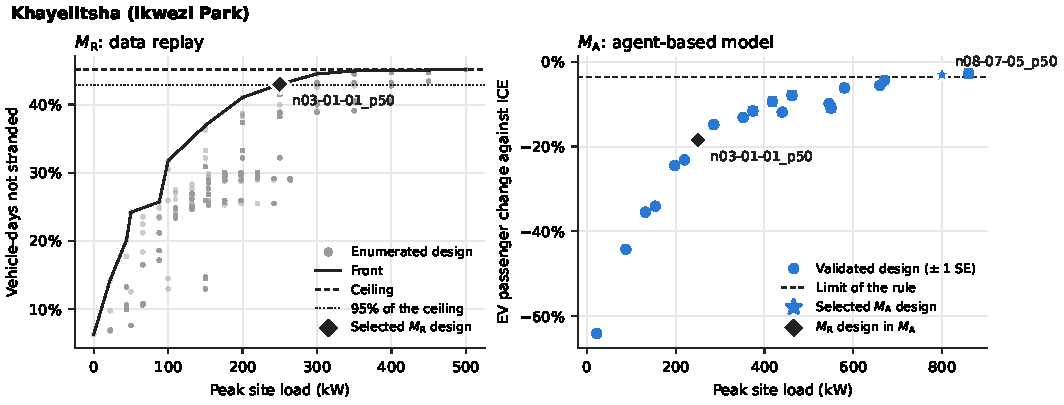
\includegraphics[width=\textwidth]{figures/fig02_design_space_a.pdf}\\[0.5em]
    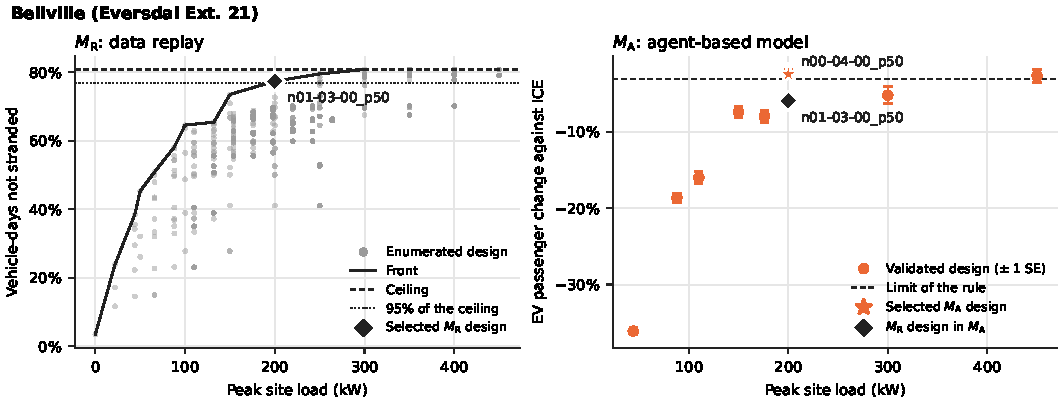
\includegraphics[width=\textwidth]{figures/fig02_design_space_b.pdf}\\[0.5em]
    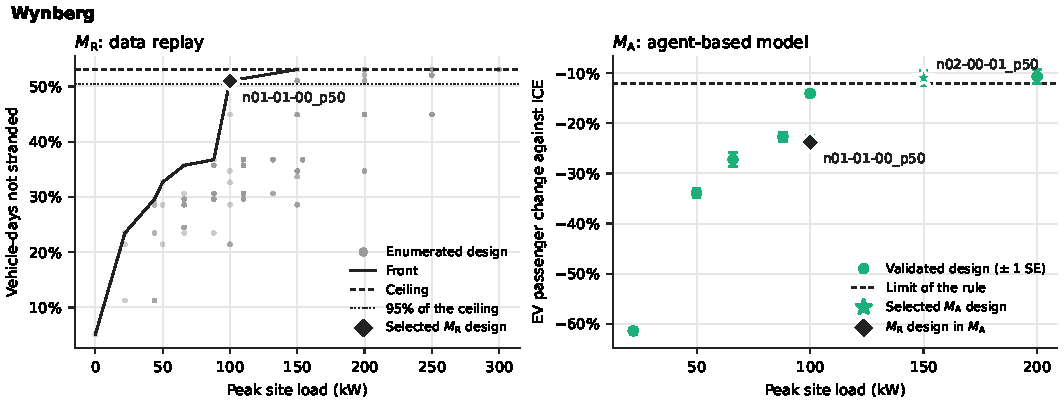
\includegraphics[width=\textwidth]{figures/fig02_design_space_c.pdf}
    \caption{Design space of each community in both models, each in its model-native objectives: (a) Khayelitsha, (b) Bellville, (c) Wynberg. Left, \MR: every enumerated design (grey), the front (line), the ceiling of the not-stranded share (dashed) and 95\% of it (dotted), and the selected \MR{} design (diamond). Right, \MA: the validated designs (mean $\pm$ one standard error over five seeds), the limit of the one-standard-error rule (dashed), the selected \MA{} design (star) and the \MR{} design evaluated in \MA{} (diamond).}
    \label{fig:design_space}
\end{figure}

\begin{table}[htbp]
    \centering
    \footnotesize
    \caption{Design that each model selects in each community: the connectors $N_1$, $N_2$ and $N_3$ at the first three hubs, the power $P$ of a connector, the installed power and the peak site load. A design ID $n\,N_1$-$N_2$-$N_3$\_$p\,P$ gives the same values.}
    \label{tab:selected_designs}
    % Source: tab06_selected_designs.
    \begin{tabularx}{\linewidth}{@{}XlXrrrrrr@{}}
        \toprule
        \textbf{Community} & Model & Design & $N_1$ & $N_2$ & $N_3$ & $P$ (kW) & Installed (kW) & Peak (kW) \\
        \midrule
        Khayelitsha & \MR & n03-01-01\_p50 & 3 & 1 & 1 & 50 & 250 & 250 \\
                    & \MA & n08-07-05\_p50 & 8 & 7 & 5 & 50 & 1,000 & 800 \\
        \addlinespace
        Bellville   & \MR & n01-03-00\_p50 & 1 & 3 & 0 & 50 & 200 & 200 \\
                    & \MA & n00-04-00\_p50 & 0 & 4 & 0 & 50 & 200 & 200 \\
        \addlinespace
        Wynberg     & \MR & n01-01-00\_p50 & 1 & 1 & 0 & 50 & 100 & 100 \\
                    & \MA & n02-00-01\_p50 & 2 & 0 & 1 & 50 & 150 & 150 \\
        \bottomrule
    \end{tabularx}
\end{table}

\subsection{Consequences of the replay design}
% Discuss > RQ3 (Table~\ref{tab:cross_evaluation}) -> The M_R design against the M_A design in M_A. Preliminary: the M_R design loses more EV passengers (Wynberg -12.9 points, SE 0.6; Khayelitsha -15.4 points, SE 0.8), with a lower peak site load and less site energy.
% Discuss > Where the passengers go -> The expired share and the wait do not change between designs: the passengers that the EVs lose go to the ICE vehicles. This loss is invisible in an all-request service measure and in M_R.

\begin{table}[htbp]
    \centering
    \footnotesize
    \caption{Selected \MR{} design against the selected \MA{} design, both evaluated in \MA: the means over five validation seeds, the difference (\MR{} design minus \MA{} design) and its standard error (SE) over the paired seeds. The EV passenger change compares the passengers of the EV agents with the same agents as internal-combustion vehicles on the same seed; the passenger loss $\ell$ also corrects for their time away from home.}
    \label{tab:cross_evaluation}
    % Source: tab07_cross_evaluation.
    \begin{tabularx}{\linewidth}{@{}Xrrrr@{}}
        \toprule
        \textbf{Measure} & \MR{} design & \MA{} design & Difference & SE \\
        \midrule
        \multicolumn{5}{@{}l}{\textit{Khayelitsha}} \\
        EV passenger change against ICE & $-$0.185 & $-$0.030 & $-$0.154 & 0.008 \\
        EV passenger loss $\ell$ & 0.192 & 0.032 & 0.160 & 0.007 \\
        Expired requests (share) & 0.041 & 0.041 & 0.000 & 0.000 \\
        Mean passenger wait (s) & 125.4 & 122.9 & 2.6 & 0.7 \\
        Peak site load (kW) & 250 & 800 & $-$550 & 15.8 \\
        Site energy (kWh a day) & 3,797 & 5,012 & $-$1,215 & 34.6 \\
        Site sessions a day & 237.9 & 343.6 & $-$105.7 & 1.8 \\
        Stranded EV-days (share) & 0.000 & 0.000 & 0.000 & 0.000 \\
        \addlinespace
        \multicolumn{5}{@{}l}{\textit{Bellville}} \\
        EV passenger change against ICE & $-$0.060 & $-$0.025 & $-$0.035 & 0.011 \\
        EV passenger loss $\ell$ & 0.053 & 0.021 & 0.032 & 0.006 \\
        Expired requests (share) & 0.049 & 0.049 & 0.000 & 0.000 \\
        Mean passenger wait (s) & 268.1 & 270.9 & $-$2.8 & 3.0 \\
        Peak site load (kW) & 200 & 200 & 0 & 0.0 \\
        Site energy (kWh a day) & 1,819 & 1,925 & $-$105 & 25.6 \\
        Site sessions a day & 124.3 & 131.2 & $-$6.8 & 2.8 \\
        Stranded EV-days (share) & 0.000 & 0.000 & 0.000 & 0.000 \\
        \addlinespace
        \multicolumn{5}{@{}l}{\textit{Wynberg}} \\
        EV passenger change against ICE & $-$0.238 & $-$0.109 & $-$0.129 & 0.006 \\
        EV passenger loss $\ell$ & 0.252 & 0.118 & 0.134 & 0.005 \\
        Expired requests (share) & 0.033 & 0.034 & 0.000 & 0.001 \\
        Mean passenger wait (s) & 1,006.0 & 1,015.3 & $-$9.4 & 11.9 \\
        Peak site load (kW) & 100 & 150 & $-$50 & 0.0 \\
        Site energy (kWh a day) & 1,196 & 1,444 & $-$247 & 23.1 \\
        Site sessions a day & 62.0 & 86.0 & $-$24.0 & 1.8 \\
        Stranded EV-days (share) & 0.000 & 0.000 & 0.000 & 0.000 \\
        \bottomrule
    \end{tabularx}
\end{table}

\subsection{Sensitivity and consistency across communities}
% Discuss > Sensitivity (Figure~\ref{fig:sensitivity}, Table~\ref{tab:sensitivity}) -> The EV passenger change of both designs in each case. Does the M_A design stay better than the M_R design in every case? Preliminary for Wynberg: yes in all six cases.
% Discuss > Synthesis (Table~\ref{tab:synthesis}) -> The direction and size of each difference in each community. Three communities do not give a statistical generalisation.

\begin{figure}[htbp]
    \centering
    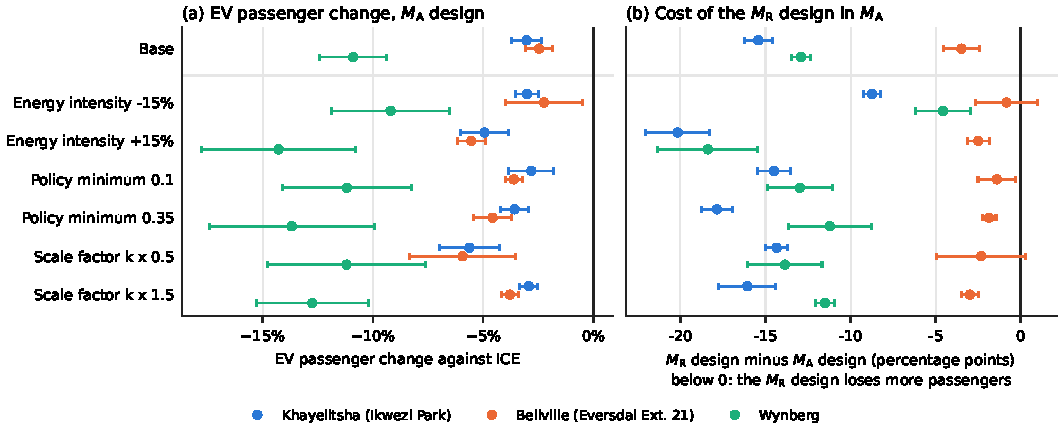
\includegraphics[width=\textwidth]{figures/fig03_sensitivity.pdf}
    \caption{Sensitivity of the EV passenger change in \MA{} in each community (colour). (a) EV passenger change against internal-combustion operation of the selected \MA{} design. (b) EV passenger change of the selected \MR{} design minus that of the selected \MA{} design, both evaluated in \MA{}, in percentage points; below zero, the \MR{} design loses more passengers. Mean $\pm$ one standard error over three seeds in each case and five in the base case.}
    \label{fig:sensitivity}
\end{figure}

\begin{table}[htbp]
    \centering
    \footnotesize
    \caption{Sensitivity of the selected \MA{} and \MR{} designs, both evaluated in \MA: (a) the EV passenger change against internal-combustion operation and (b) the stranded share of the EV-days. Means over three seeds; the base case uses the five validation seeds.}
    \label{tab:sensitivity}
    % Source: tab08_sensitivity.
    \begin{tabularx}{\linewidth}{@{}Xrrrrrr@{}}
        \toprule
        & \multicolumn{2}{c}{Khayelitsha} & \multicolumn{2}{c}{Bellville} & \multicolumn{2}{c}{Wynberg} \\
        \cmidrule(lr){2-3}\cmidrule(lr){4-5}\cmidrule(l){6-7}
        \textbf{Case} & \MA{} design & \MR{} design & \MA{} design & \MR{} design & \MA{} design & \MR{} design \\
        \midrule
        \multicolumn{7}{@{}l}{\textit{(a) EV passenger change against ICE}} \\
        Base & $-$0.030 & $-$0.185 & $-$0.025 & $-$0.060 & $-$0.109 & $-$0.238 \\
        Energy intensity $-15\%$ & $-$0.030 & $-$0.118 & $-$0.022 & $-$0.031 & $-$0.092 & $-$0.138 \\
        Energy intensity $+15\%$ & $-$0.049 & $-$0.251 & $-$0.055 & $-$0.080 & $-$0.143 & $-$0.327 \\
        Policy minimum 0.1 & $-$0.028 & $-$0.173 & $-$0.036 & $-$0.050 & $-$0.112 & $-$0.242 \\
        Policy minimum 0.35 & $-$0.036 & $-$0.214 & $-$0.046 & $-$0.064 & $-$0.137 & $-$0.249 \\
        Scale factor $k \times 0.5$ & $-$0.056 & $-$0.200 & $-$0.059 & $-$0.083 & $-$0.112 & $-$0.251 \\
        Scale factor $k \times 1.5$ & $-$0.029 & $-$0.190 & $-$0.038 & $-$0.068 & $-$0.127 & $-$0.243 \\
        \addlinespace
        \multicolumn{7}{@{}l}{\textit{(b) Stranded EV-days (share)}} \\
        Base & 0.000 & 0.000 & 0.000 & 0.000 & 0.000 & 0.000 \\
        Energy intensity $-15\%$ & 0.000 & 0.000 & 0.000 & 0.000 & 0.000 & 0.000 \\
        Energy intensity $+15\%$ & 0.000 & 0.000 & 0.000 & 0.000 & 0.000 & 0.000 \\
        Policy minimum 0.1 & 0.000 & 0.000 & 0.001 & 0.001 & 0.000 & 0.000 \\
        Policy minimum 0.35 & 0.000 & 0.000 & 0.000 & 0.000 & 0.000 & 0.000 \\
        Scale factor $k \times 0.5$ & 0.000 & 0.000 & 0.000 & 0.000 & 0.000 & 0.000 \\
        Scale factor $k \times 1.5$ & 0.000 & 0.000 & 0.000 & 0.000 & 0.000 & 0.000 \\
        \bottomrule
    \end{tabularx}
\end{table}

\begin{table}[htbp]
    \centering
    \footnotesize
    \caption{Direction and size of each difference between the models in each community: whether the two models select the same design, the installed power of the \MA{} design minus that of the \MR{} design, and the EV passenger change of the \MR{} design minus that of the \MA{} design in \MA{} with its standard error (equal within two standard errors). Three communities do not give a statistical generalisation.}
    \label{tab:synthesis}
    % Source: tab09_synthesis.
    \begin{tabularx}{\linewidth}{@{}Xllcrlrl@{}}
        \toprule
        & \multicolumn{2}{c}{Selected design} & & \multicolumn{2}{c}{Installed power} & \multicolumn{2}{c}{EV passenger change} \\
        \cmidrule(lr){2-3}\cmidrule(lr){5-6}\cmidrule(l){7-8}
        \textbf{Community} & \MR & \MA & Same & Difference (kW) & Direction & Difference (SE) & Direction \\
        \midrule
        Khayelitsha & n03-01-01\_p50 & n08-07-05\_p50 & No & +750 & Higher & $-$0.154 (0.008) & Lower \\
        Bellville & n01-03-00\_p50 & n00-04-00\_p50 & No & 0 & Equal & $-$0.035 (0.011) & Lower \\
        Wynberg & n01-01-00\_p50 & n02-00-01\_p50 & No & +50 & Higher & $-$0.129 (0.006) & Lower \\
        \bottomrule
    \end{tabularx}
\end{table}

% --------------------------------------------------
%   Discussion
% --------------------------------------------------

\section{Discussion}
\textcolor{red}{TODO: Complete discussion.}

\subsection{When does driver agency matter?}
% Discuss > Answer the title question from RQ1 to RQ4. Under which conditions (hub charging binding, competition density k) the two models select different designs.

\subsection{Implications for electrification pilots}
% Discuss > Chargers at formal termini (ten of eleven main hubs are within 200 m of one). Hub charging load in the grid peaks. The mixed-fleet penalty for the first EVs and what it means for operators and for pilot design.

\subsection{Limitations}
\label{sec:discussion_limitations}
% Discuss > Selection on the outcome (the screening is a simple replay); communities are spatial territories, not associations or owners; mixed membership (LDA ARI 0.36); most \MA{} agents are synthetic and Sebenza routers are in partner vehicles; uncertainty of k (AM peak, 2022 survey, few corridors); the gap rule; small samples; three cases do not give a statistical generalisation; the \MA{} limits in the reproduction of passenger service; a two-week December window.

\subsection{Future work}
% Discuss > More communities and seasons, multiple sites per community, behavioural data on charging decisions, grid-aware charging.

% --------------------------------------------------
%   Conclusion
% --------------------------------------------------

\section{Conclusion}
\textcolor{red}{TODO: Complete conclusion.}

\bibliographystyle{elsarticle-num-names}
\bibliography{references}

% --------------------------------------------------
%   Appendices
% --------------------------------------------------

\appendix

\section{Validation of the vehicle communities}
\label{app:communities}
% Discuss > Evidence tests (communities.md 4.5) -> Null model (100 randomised fleets by curveball trades; modularity z and p), seed stability (median ARI of 50 seeds), temporal stability (early against late dates, ARI and NMI) and view agreement (each view against the combined partition). Take the values of the accepted partition from evidence.parquet; the values of the earlier runs are of replaced partitions.
% Discuss > Resolution sweep -> Corridor containment and stability for each resolution. The partition is sensitive to the network near the 90% containment target (0.5 and 0.75); Bellville is selected under both.

\section{Network construction and coverage}
\label{app:network}
% Discuss > Support sweep (the support rule controls the captured events and dwell, not the represented distance) and pass-radius sweep (50, 100 and 150 m give a represented distance of 63.6%, 66.8% and 68.5%); the review queue (candidate cells, doubtful edges and formal/support conflicts; the speed rule only for edges with a median travel time of 160 s or more) and its decisions; the close-node distance (300 m, from a comparison of 300, 400 and 500 m).
% Discuss > Coverage measures -> Captured events and dwell, represented distance between stops, and the reasons for lost distance.

\section{Agent-based model specification}
\label{app:abm}
% Discuss > ODD description of parasim-engine as configured (docs/model-agent-based.md): entities, process overview, route choice, stopping and boarding, demand, charging, memory, stochasticity and observation.
% Discuss > Engine corrections made in the study (a connector only when the policy says charge and the shift has not ended; the energy of the last charging step counts; the route energy test and the charge before going home; charging continues below the need of the cheapest route; no route that a full battery cannot finish): what each corrects, and that the ICE logs stay identical.

\section{Calibration targets and search}
\label{app:calibration}
% Discuss > Target values, noise and floors for each community. Strategy files with their SHA-256 values, parameters, bounds and budgets. The traffic-light assessment and the hold-out reports.

% TODO: The Bluedot replication is not part of the new pipeline (the study uses only the Sebenza Cape Town fleet). Rerun it with the same steps, or remove this appendix.
\section{Replication with a second fleet}
% Discuss > Bluedot, November 2022 (28 days, 621 vehicles, 05:00--20:00 only): 23 communities, seed ARI 1.0, early and late ARI 0.92; screening classes. Night is not observed, so overnight-only viability is optimistic.

\section{Reproducibility}
\label{app:reproducibility}
% Discuss > The 13 steps, their manifests (input, settings, code and output digests) and the human decision of each step, mapped to the sections of this paper. The parasim-engine commit and the SHA-256 of the engine executable in the experiments inputs. No paths, pseudonyms or coordinates.

\end{document}
